\documentclass{sig-alternate}
\pdfpagewidth=8.5in
\pdfpageheight=11in
\special{papersize=8.5in,11in}

%%%%%%%%%%%%%%%%%%%%%%%%%%%%%%%%%%%%%%%%%%%%%%%%%%%%%%
% Packages
\usepackage{bm}
\usepackage{graphicx}
\usepackage{tabularx}
\usepackage[dvipsnames]{xcolor}
\usepackage{xspace}
\usepackage{float}
\usepackage{rotating}
\usepackage{xstring} % for string operations
\usepackage{wasysym} % Table legend with symbols input from post-processing
\usepackage{MnSymbol} % Table legend with symbols input from post-processing
%\usepackage[hidelinks]{hyperref} % make COCO papers clickable

%%%%%%%%%%%%%%%%%%%%%%%%%%%%%%%%%%%%%%%%%%%%%%%%%%%%%%
% Definitions

% Algorithm names as they appear in the tables, uncomment if necessary
%\newcommand{\algAtables}{\algaperfprof}  % first argument in the post-processing
%\newcommand{\algBtables}{\algbperfprof}  % first argument in the post-processing
%\newcommand{\algCtables}{\algcperfprof}  % first argument in the post-processing
%\newcommand{\algDtables}{\algdperfprof}  % second argument in the post-processing
%\newcommand{\algEtables}{\algeperfprof}  % second argument in the post-processing
% location of pictures files
\newcommand{\bbobdatapath}{comparison/}
\input{\bbobdatapath bbob_pproc_commands.tex}
\graphicspath{{\bbobdatapath}}
\newcommand{\algname}{IBEA}

%%%%%%%%%%%%%%%%%%%%%%%%%%%%%%%%%%%%%%%%%%%%%%%%%%%%%%
% pre-defined commands
\newcommand{\DIM}{\ensuremath{\mathrm{DIM}}}
\newcommand{\aRT}{\ensuremath{\mathrm{aRT}}}
\newcommand{\FEvals}{\ensuremath{\mathrm{FEvals}}}
\newcommand{\nruns}{\ensuremath{\mathrm{Nruns}}}
\newcommand{\Df}{\ensuremath{\Delta f}}
\newcommand{\DI}{\ensuremath{\Delta I}}
\newcommand{\nbFEs}{\ensuremath{\mathrm{\#FEs}}}
\newcommand{\fopt}{\ensuremath{f_\mathrm{opt}}}
\newcommand{\ftarget}{\ensuremath{f_\mathrm{t}}}
\newcommand{\Itarget}{\ensuremath{I_\mathrm{target}}}
\newcommand{\CrE}{\ensuremath{\mathrm{CrE}}}
\newcommand{\change}[1]{{\color{red} #1}}
\newcommand{\bbobbiobj}{{\ttfamily bbob-biobj}\xspace}
\newcommand{\hvref}{I^{\mathrm{ref}}}
\newcommand{\TODO}[1]{{\color{red} TODO: #1}}

    \renewcommand{\topfraction}{1}	% max fraction of floats at top
    \renewcommand{\bottomfraction}{1} % max fraction of floats at bottom
    %   Parameters for TEXT pages (not float pages):
    \setcounter{topnumber}{3}
    \setcounter{bottomnumber}{3}
    \setcounter{totalnumber}{3}     % 2 may work better
    \setcounter{dbltopnumber}{4}    % for 2-column pages
    \renewcommand{\dbltopfraction}{1}	% fit big float above 2-col. text
    \renewcommand{\textfraction}{0.0}	% allow minimal text w. figs
    %   Parameters for FLOAT pages (not text pages):
    \renewcommand{\floatpagefraction}{0.80}	% require fuller float pages
    % N.B.: floatpagefraction MUST be less than topfraction !!
    \renewcommand{\dblfloatpagefraction}{0.7}	% require fuller float pages

%%%%%%%%%%%%%%%%%%%%%%%%%%%%%%%%%%%%%%%%%%%%%%%%%%%%%%

\begin{document}

\IfFileExists{\bbobdatapath ppfig2_f001.pdf}{2 algorithms currently not supported}{}

\title{Benchmarking of the Indicator-based evolution algorithm using the Bi-Objective BBOB Test Suite
% \titlenote{If needed}
}
\subtitle{Final report
\titlenote{Submission deadline: October 21st.}}

\numberofauthors{5}
\author{
\alignauthor 
Daro Heng
\alignauthor
Karim Kouki
\alignauthor
Ahmed Mazari
\and
\alignauthor 
Mihaela Sorostinean
\alignauthor 
Aris Tritas
}

\maketitle
\begin{abstract}
The objective of this project was to study, implement and benchmark the Indicator Based Evolutionary Algorithm \\ (IBEA) using  the Comparing Continuous Optimizer (COCO) platform. Firstly we provide a brief overview of the algorithm. Secondly, we describe our implementation and experimental setup. Finally, we discuss the obtained results and compare them to both baseline approaches and related work.
\end{abstract}

\section{Setting}
In the context of a multi-objective optimization, the main goal is to find a good approximation of the set of Pareto-optimal solutions.
An evolutionary algorithm is an exploration strategy of the domain space $\mathbb{R}^n$ which seeks optimal solution vectors defined in the objective space $\mathbb{R}^k$ (here $k=2$) by promoting at each generation the fittest and/or the  newest individuals from a population of decision vectors.

The performance measure used by IBEA for determining the relative quality of two solution sets in the objective space is a binary indicator function $I: \Omega \times \Omega \rightarrow \mathbb{R}$. 
In terms of two decision vectors $\bm{x}^1$ and $\bm{x}^2$,  the domination relation is defined as : $\bm{x}^1 \succ \bm{x}^2 \leftrightarrow ( f_i(\bm{x}^1) \leq f_i(\bm{x}^2) \; \forall i \in \{1, ..., n\} \;\text{and}\; f_j(\bm{x}^1) < f_j(\bm{x}^2)$ for at least one objective$)$. 
The epsilon indicator, which is compliant with this domination relationship, is defined for pairwise comparisons as: $$I_{\epsilon^+} (\{\bm{x}^1\}, \{\bm{x}^2\}) = \min_\epsilon f_i(\bm{x}^1) - \epsilon \leq f_i(\bm{x}^2) \; \forall i \in \{1, ..., n\}$$. 
Its focus is to summarize the minimum distance needed to improve on the Pareto set approximation to a single scalar. 
Intuitively, the reduction to a single scalar may incur a  loss of information regarding some dimensions of objective space. Indeed, the fact that the indicator chooses the minimum improvement across all objectives implies \emph{conservative} rather than more \emph{optimistic} updates of the fitness estimate. Clearly, we may miss out on potential improvement on some of the targeted objectives. The fitness value is defined in the sequel as a measure of the usefulness of each individual with regards to the optimization goal. As such, the algorithm tries to maximize it.
$$ F(\bm{x}^1) = \sum_{\bm{x}^2 \in P \setminus \{\bm{x}^1\}} - \exp{\frac{I(\{\bm{x}^1\}, \{\bm{x}^2\})}{\kappa}}$$ where $P$ is the population set, and $\bm{x} \in \mathbb{R}^n$. The fitness function of an approximation set is defined as a \emph{dominance preserving relation}.

Moreover, as the optimization functions are typically unnormalized, IBEA scales both the values taken by the objective function as well as the values taken by the indicator function. Consequently the need for parameter tuning in face of problem and indicator function diversity is decreased.

\section{Implementation}
The input of the algorithm is the size of the population ($\alpha$), a maximum number of generations, a budget in function evaluations, and a fitness scaling factor ($\kappa$). The output of the algorithm is an approximation of the Pareto-set.
\begin{enumerate}
\item \textbf{Initialization:} generate an initial population P of given size uniformly between the lower and upper bound of the domain space.

\item \textbf{Fitness assignment:} compute and assign a fitness value to each individual in P.

\item \textbf{Environmental selection:} detect and remove individuals which have the smallest fitness values from the population until the current size of the population P does not exceed $\alpha$. Update the fitness values for all remaining individuals.

\item \textbf{Termination:} after the environmental selection is performed, the termination criterion of the algorithm is checked; if the maximum number of generations is reached or another termination criterion is met, the algorithm returns the set of decision vectors A.

\item \textbf{Mating Selection:} consists in creating as temporary mating pool P' which is filled with individuals from P by performing binary tournament selection with replacement on P.

\item \textbf{Variation:} finally the variation step consists applying recombination and mutation operators to the previously created mating pool.  
The offspring resulting from variation is added to P and the generation counter is incremented. The algorithm is then performed again from step 2, until a termination criterion is met.

\end{enumerate}

Population-related data (i.e decision vectors, objective and fitness values) is stored in a hash table for timely access. 
All numerical computation is done with NumPy. 
The optimizer is an object which incurs some overhead in Python. Except for the recombination and mutation operators which were implemented in separate functions to achieve modularity during testing, the optimizer is essentially a single inlined function.

\subsection{Recombination}

At first, the crossover operators we experimented with were intermediate weighting and discrete recombination. Then we implemented the Simulated Binary Crossover \cite{deb1994simulated}. The results reported here used SBX-5 for recombination.

\subsection{Variation}

For the mutation step, we began by simply adding isotropic Gaussian noise with fixed variance to the produced offspring. However, it is well known that fixed variance does not produce the fastest target values search.


\subsection*{Budget pitfall} Before the intermediate report we used an extremely small budget, which had the effect of delaying  realistic benchmarking.

\section{Experimental setup}
Our idea was to evaluate the influence of hyper-parameters on the performance achieved for different function groups and in different number of dimensions. For a reasonably low budget ($10^3$) and $10^6$ to $10^9$ number of runs, we tried the following ranges for hyper-parameters (best values in bold):
\begin{itemize}
\item Population size $\in \{50, 80, \bm{100}, 150, 200\}$
\item Number of offspring $\in \{20, 30, 35, 40, \bm{50}\}$
\item Mutation probability: \textbf{low (0.1)}, high (>0.7)
\item Crossover probability $\in {[0.5, 1.0]}$ (best was $\bm{0.7}$)
\item Initial mutation step-size $\in \{1.0, 2.5, \bm{5.0}, 10, 15\}$
\item Distribution index of the SBX operator: 2 and 5
\end{itemize}

Our focus was mostly on crossover and mutation probabilities, as well as population and offspring size. Naturally, the total runtime of an experiment depends on the size of the population, the dimension of the problem and the budget. Carrying out experiments with all their combinations would be time consuming. As such, we set for a grid search approach: we fixed all parameters except one to reasonable defaults and tuned the last one by picking values from a range of interest and comparing the output of the test suite.

%%%%%%%%%%%%%%%%%%%%%%%%%%%%%%%%%%%%%%%%%%%%%%%%%%%%%%%%%%%%%%%%%%%%%%%%%%%%%%%
\section{CPU Timing}
%%%%%%%%%%%%%%%%%%%%%%%%%%%%%%%%%%%%%%%%%%%%%%%%%%%%%%%%%%%%%%%%%%%%%%%%%%%%%%%
% note that the following text is just a proposal and can/should be changed to your needs:
In order to evaluate the CPU timing of the algorithm, we have run the \algname with restarts on the entire bbob-biobj test suite \cite{biobj2016func} for $10 D$ function evaluations. The Python code was run on a Intel(R) Core(TM) i7 CPU. For a population size of 100, the time per function evaluation ranges between $2.2ms$ and $6.5ms$ depending on whether we use isotropic mutation or not.  


%%%%%%%%%%%%%%%%%%%%%%%%%%%%%%%%%%%%%%%%%%%%%%%%%%%%%%%%%%%%%%%%%%%%%%%%%%%%%%%
\section{Results}
%%%%%%%%%%%%%%%%%%%%%%%%%%%%%%%%%%%%%%%%%%%%%%%%%%%%%%%%%%%%%%%%%%%%%%%%%%%%%%%

Results of \algname\ from experiments according to \cite{hansen2016exp} and \cite{brockhoff2016biobjective} on the benchmark
functions given in \cite{biobj2016func} are presented in
Figures~\ref{fig:ECDFsingleOne}, \ref{fig:ECDFsingleTwo}. The experiments were performed with COCO \cite{hansen2016cocoplat}, version 15.4.

Presented here are comparative ECDFs on $2 D$ with two baseline algorithms: Random Search and NSGA-II. Our best configuration is also compared with the implementation of IBEA-$\epsilon$ in the C language and the implementation of IBEA with Hypervolume indicator in Python.

\subsection*{Remark}
In the aRT tables, IBEA corresponds to the following order: IBEA-$\epsilon$ in C, IBEA-$\epsilon$ in Python and IBEA-HV in Python.

\subsection{Observations}

In low dimension, we notice that the instances in which our algorithm performs moderately well is the \textbf{separable}, \textbf{moderate} and \textbf{weakly-structured} case. It fails however in the face of mutimodal and ill-conditioned functions.

Generally speaking, derandomized step-size adaptation performs better than isotropic mutation. Moreover, extreme values of variance for the isotropic mutation negatively impact the performance of the algorithm.

In higher dimensions, the trends are the same. Clearly the supplementary degrees of freedom decrease the number of targets reached.

\subsection{Comparison of isotropic and derandomized mutation operators}

With no surprise that our algorithm has a runtime of $1e{-3}$ iff the variance is adapted. gets to 10-3 on f12

\subsection{Related Work}
To an extent the comparison  as well as results of groups studing IBEA-HV is quite revealing . 
We can safely say that the $\epsilon$ indicator may be overly simplistic for the wide range of optimization functions benchmarked
We also observe that using a better indicator tends to find targets much faster.

\section*{Conclusion}
Going forward, we may think that a more advanced step-size adaptation scheme such as CMA, and also importantly a different indicator function may function well for different problems.



%%%%%%%%%%%%%%%%%%%%%%%%%%%%%%%%%%%%%%%%%%%%%%%%%%%%%%%%%%%%%%%%%%%%%%%%%%%%%%%
%%%%%%%%%%%%%%%%%%%%%%%%%%%%%%%%%%%%%%%%%%%%%%%%%%%%%%%%%%%%%%%%%%%%%%%%%%%%%%%

% ECDFs per function in dimension 10

%%%%%%%%%%%%%%%%%%%%%%%%%%%%%%%%%%%%%%%%%%%%%%%%%%%%%%%%%%%%%%%%%%%%%%%%%%%%%%%
\begin{figure*}
\centering
\begin{tabular}{@{\hspace*{-0.005\textwidth}}l@{\hspace*{-0.005\textwidth}}l@{\hspace*{-0.005\textwidth}}l@{\hspace*{-0.005\textwidth}}l@{\hspace*{-0.005\textwidth}}l@{\hspace*{-0.005\textwidth}}}
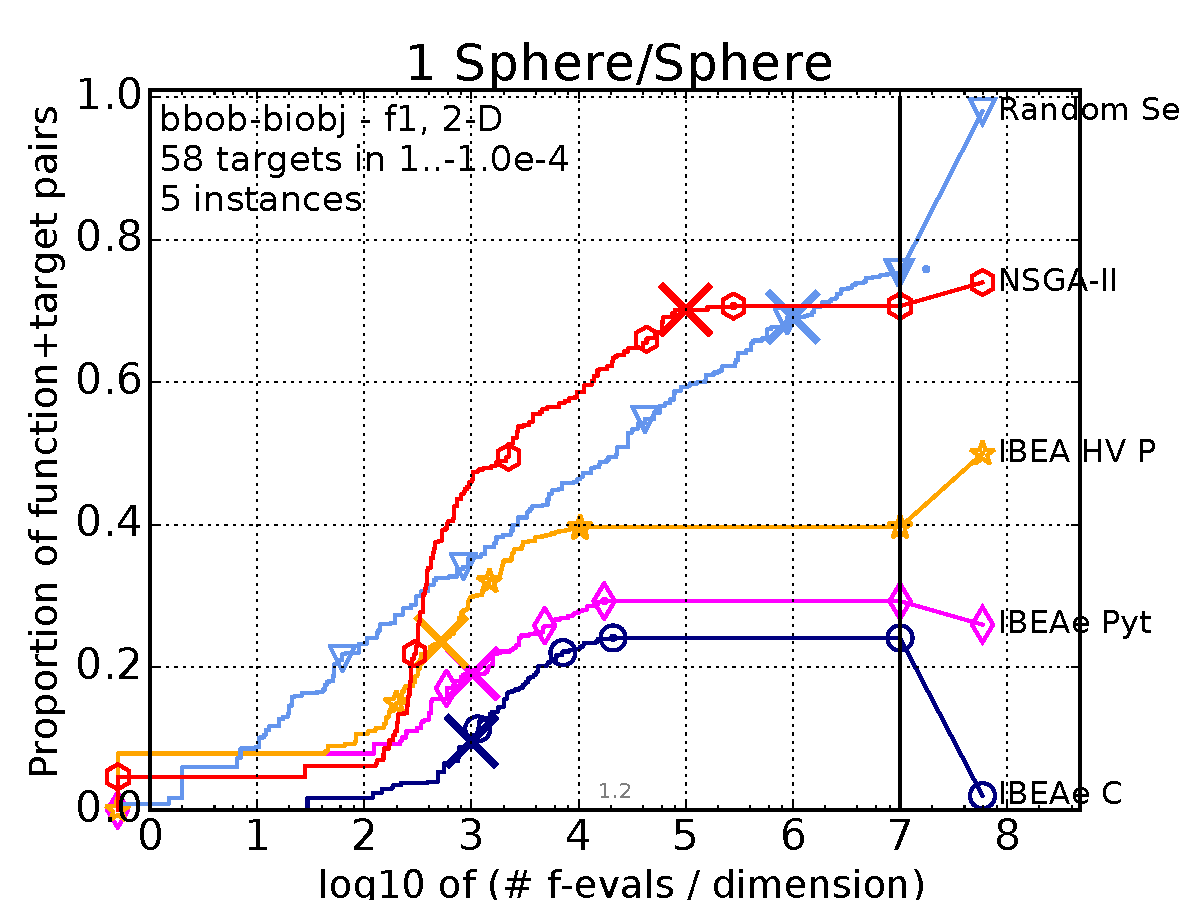
\includegraphics[width=0.2\textwidth]{pprldmany-single-functions/pprldmany_f001_02D}&
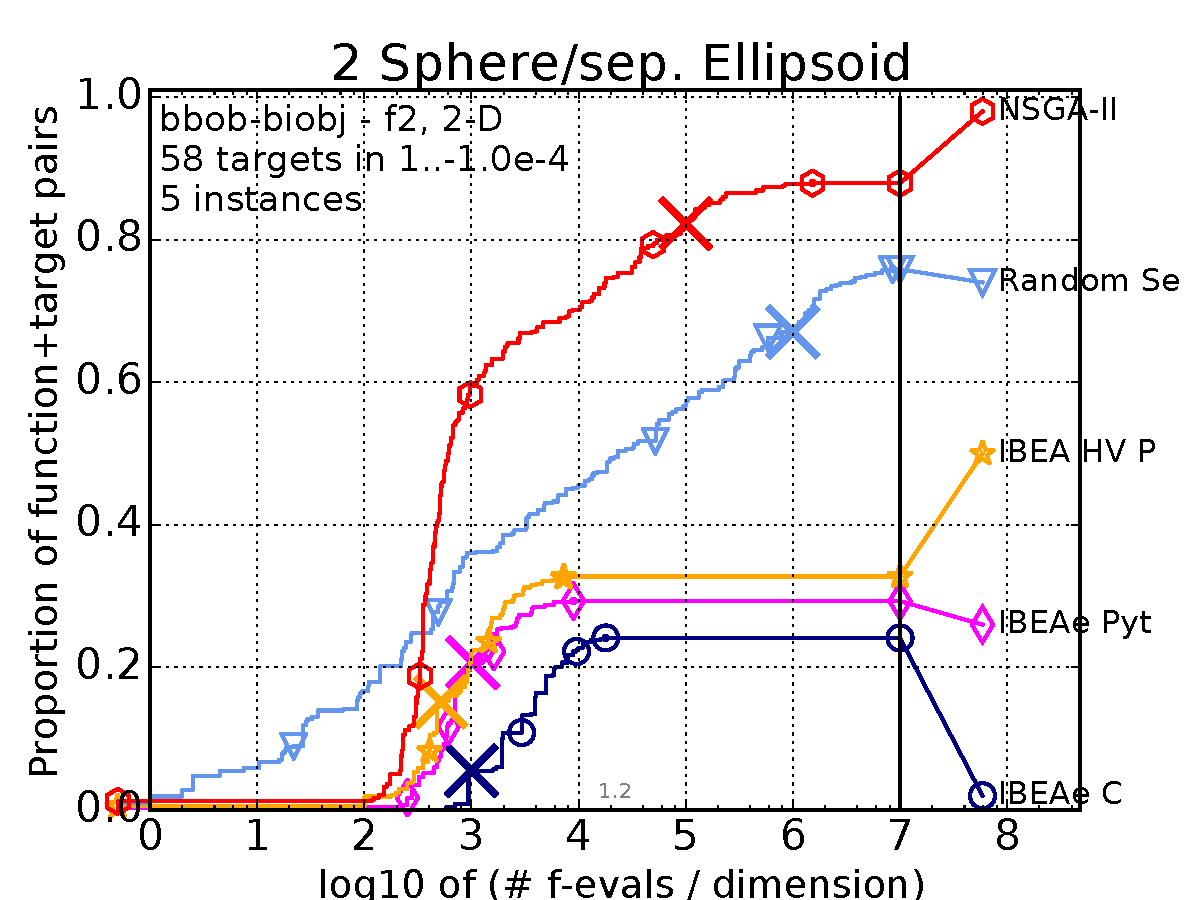
\includegraphics[width=0.2\textwidth]{pprldmany-single-functions/pprldmany_f002_02D}&
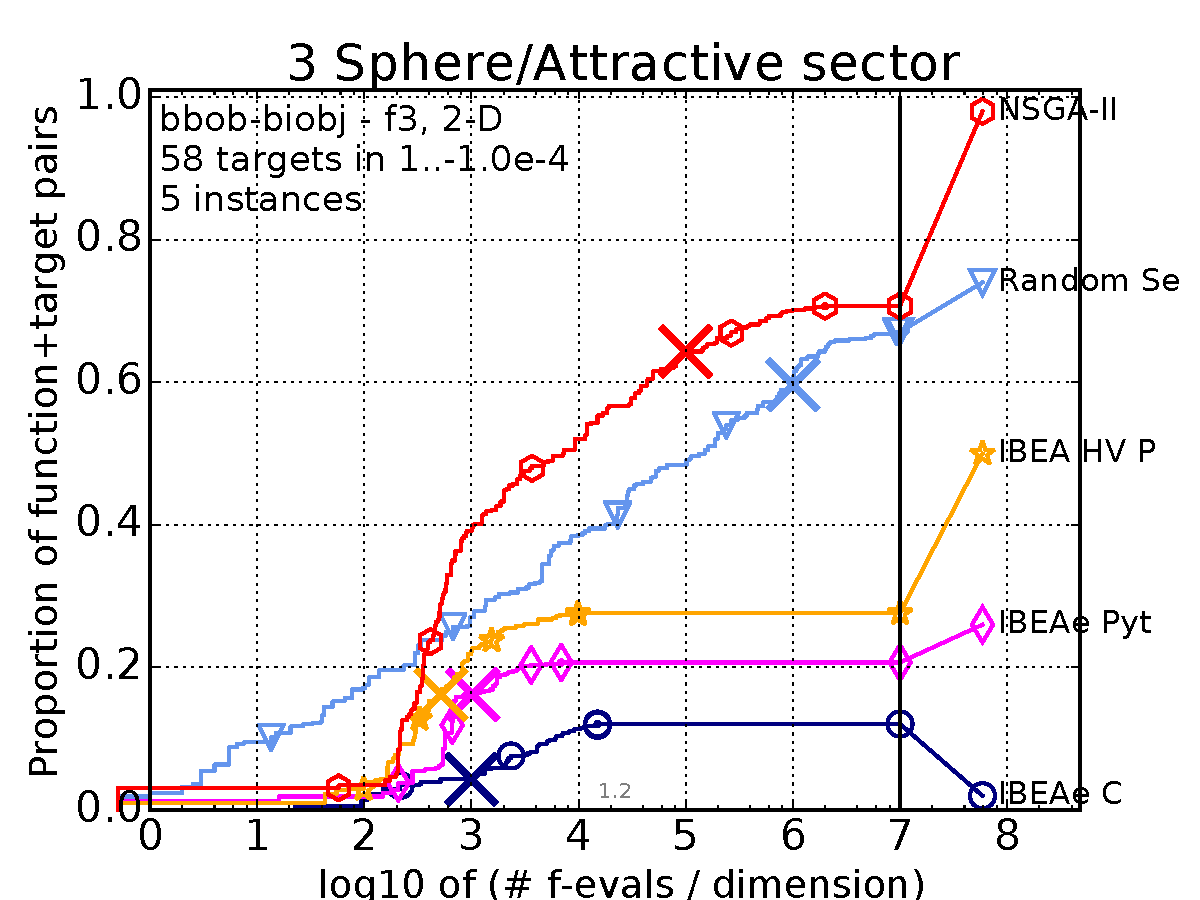
\includegraphics[width=0.2\textwidth]{pprldmany-single-functions/pprldmany_f003_02D}&
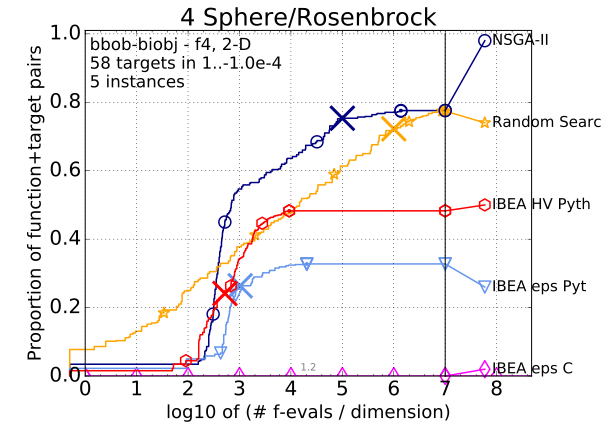
\includegraphics[width=0.2\textwidth]{pprldmany-single-functions/pprldmany_f004_02D}&
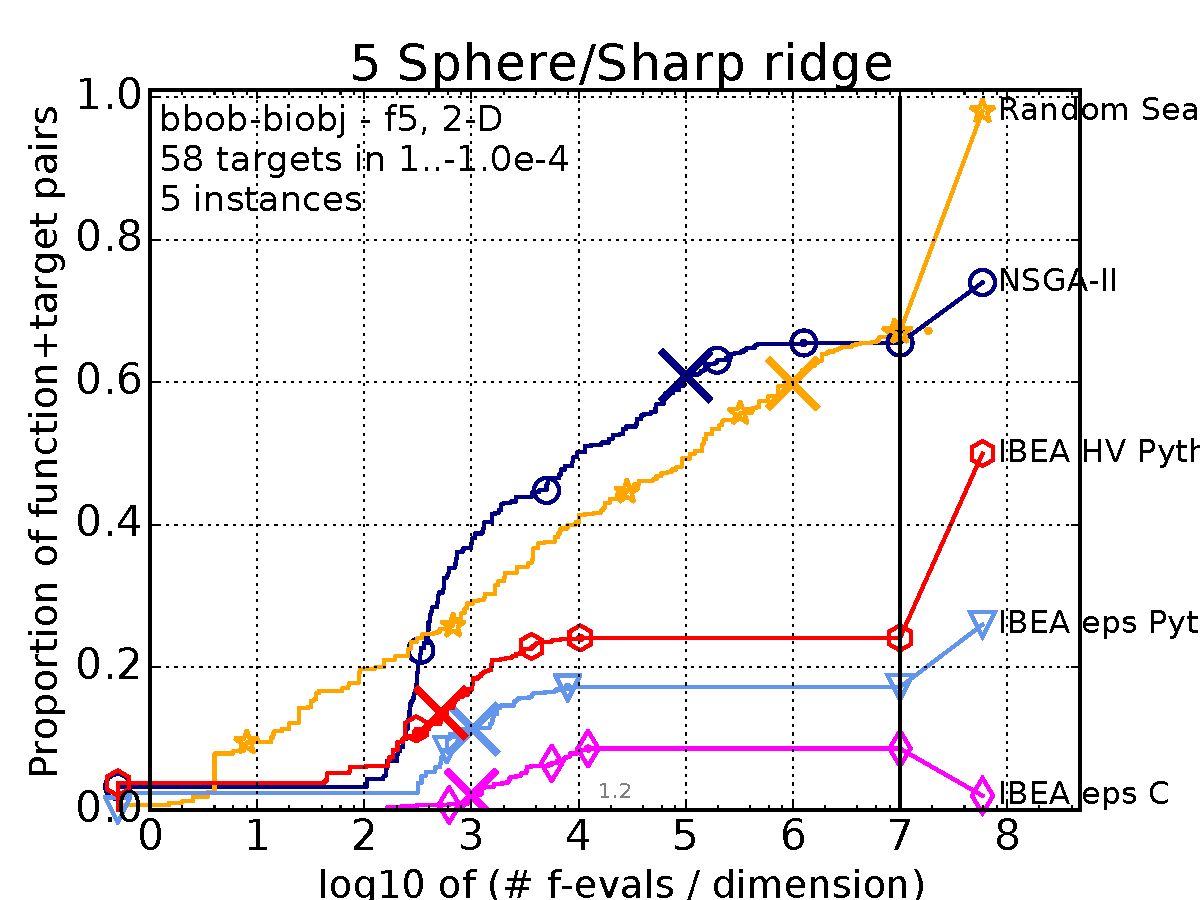
\includegraphics[width=0.2\textwidth]{pprldmany-single-functions/pprldmany_f005_02D}\\[-1.8ex]
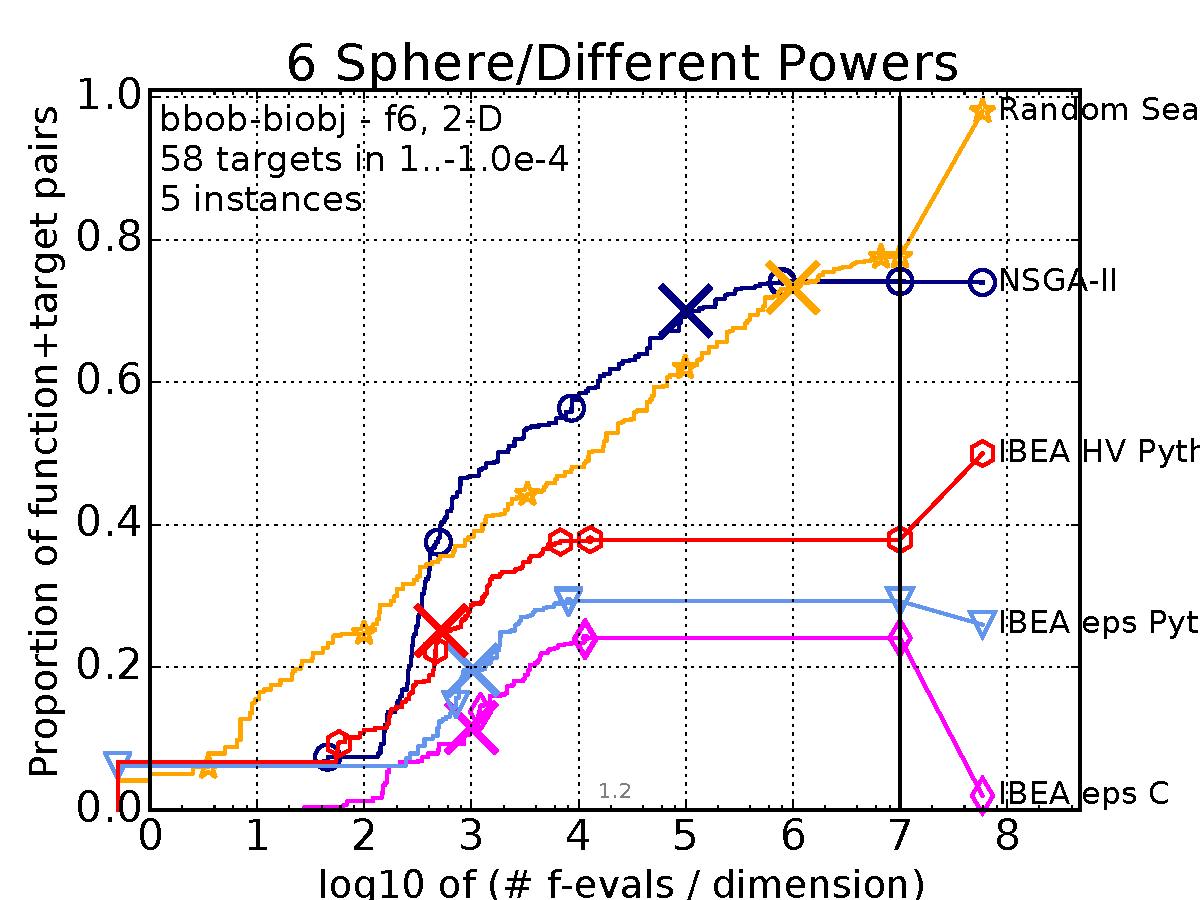
\includegraphics[width=0.2\textwidth]{pprldmany-single-functions/pprldmany_f006_02D}&
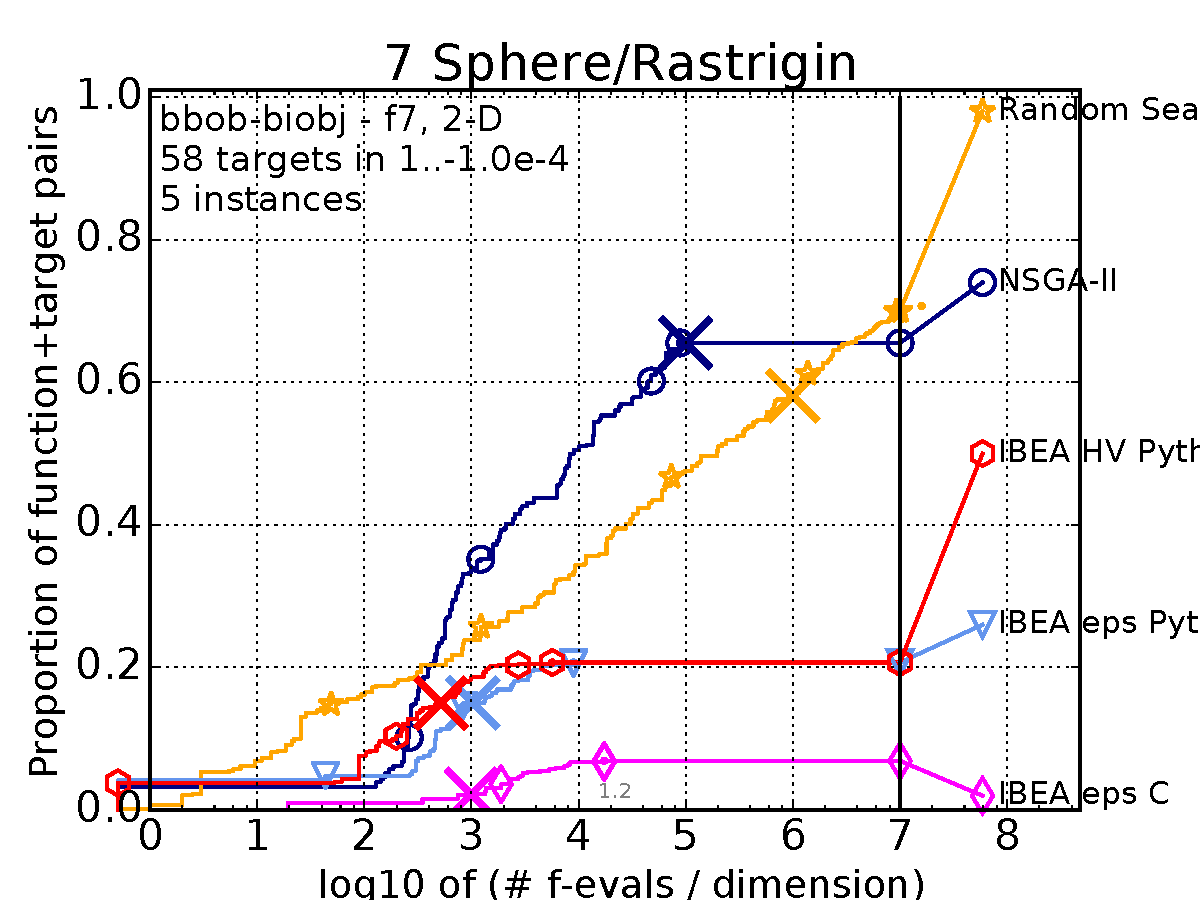
\includegraphics[width=0.2\textwidth]{pprldmany-single-functions/pprldmany_f007_02D}&
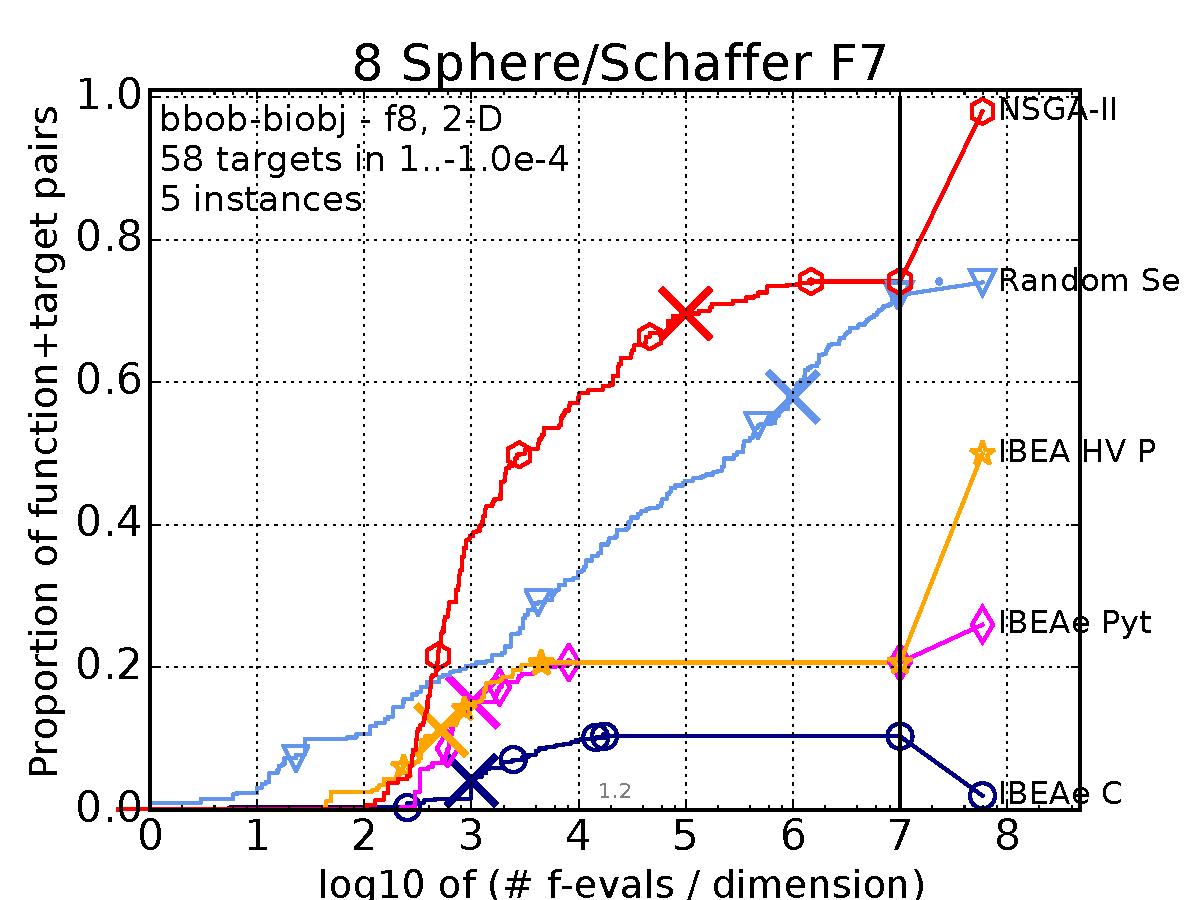
\includegraphics[width=0.2\textwidth]{pprldmany-single-functions/pprldmany_f008_02D}&
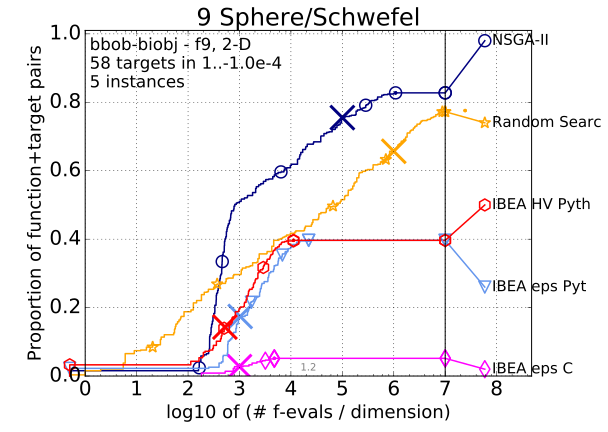
\includegraphics[width=0.2\textwidth]{pprldmany-single-functions/pprldmany_f009_02D}&
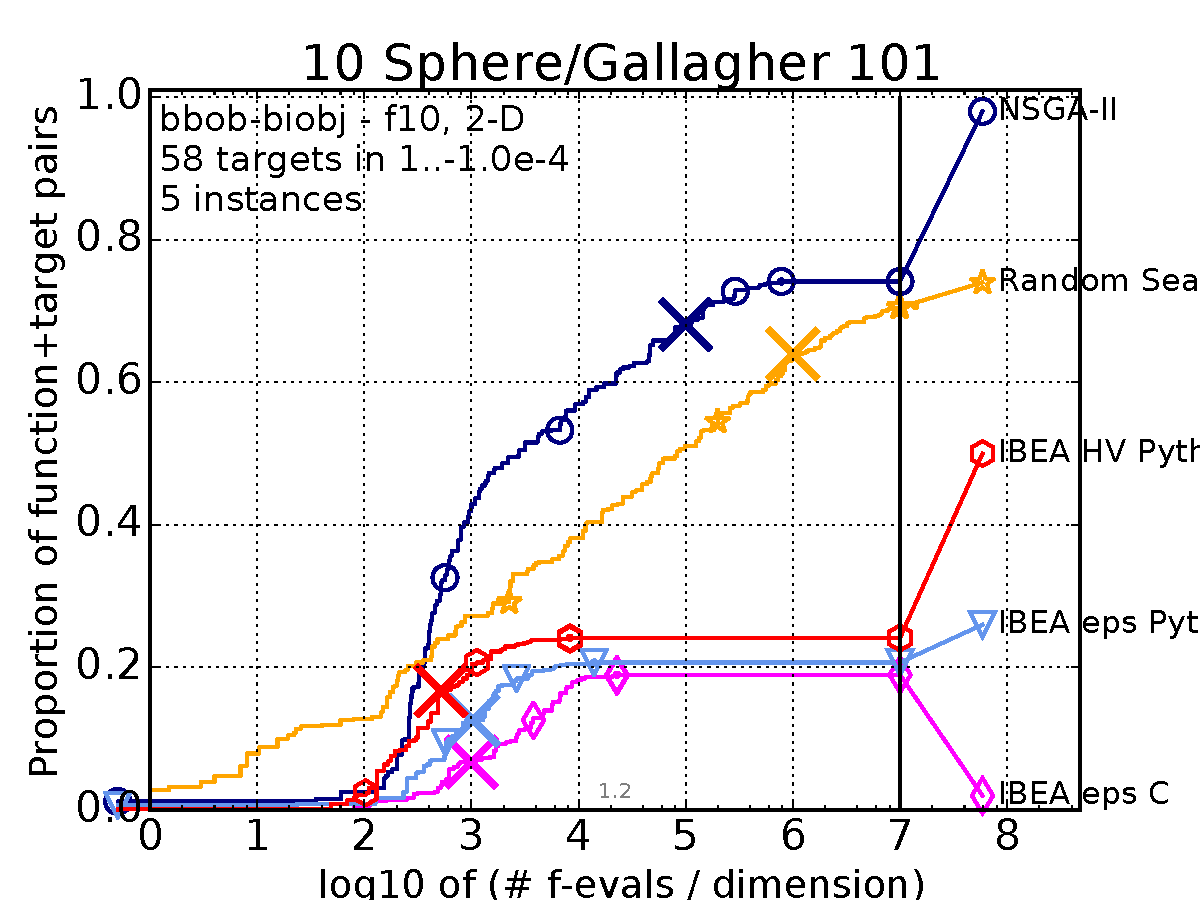
\includegraphics[width=0.2\textwidth]{pprldmany-single-functions/pprldmany_f010_02D}\\[-1.8ex]
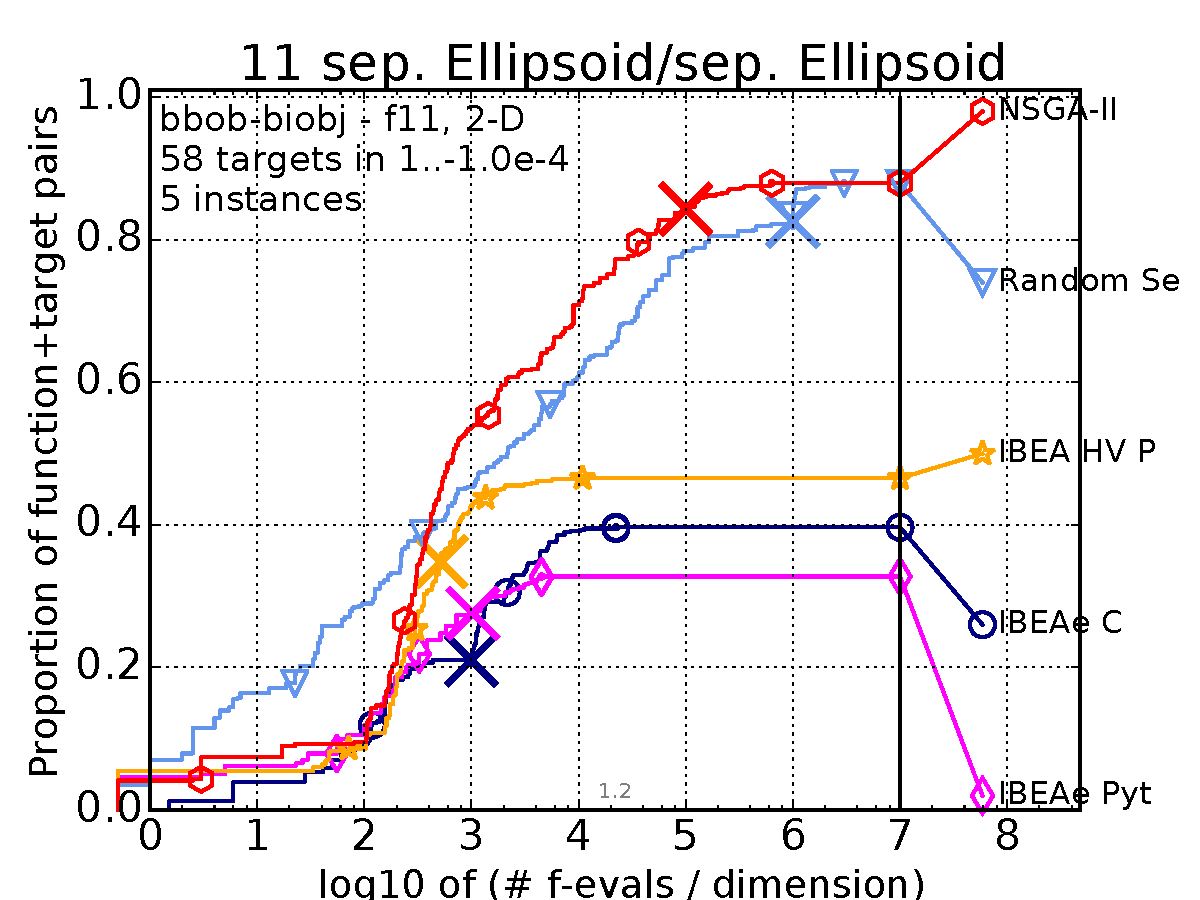
\includegraphics[width=0.2\textwidth]{pprldmany-single-functions/pprldmany_f011_02D}&
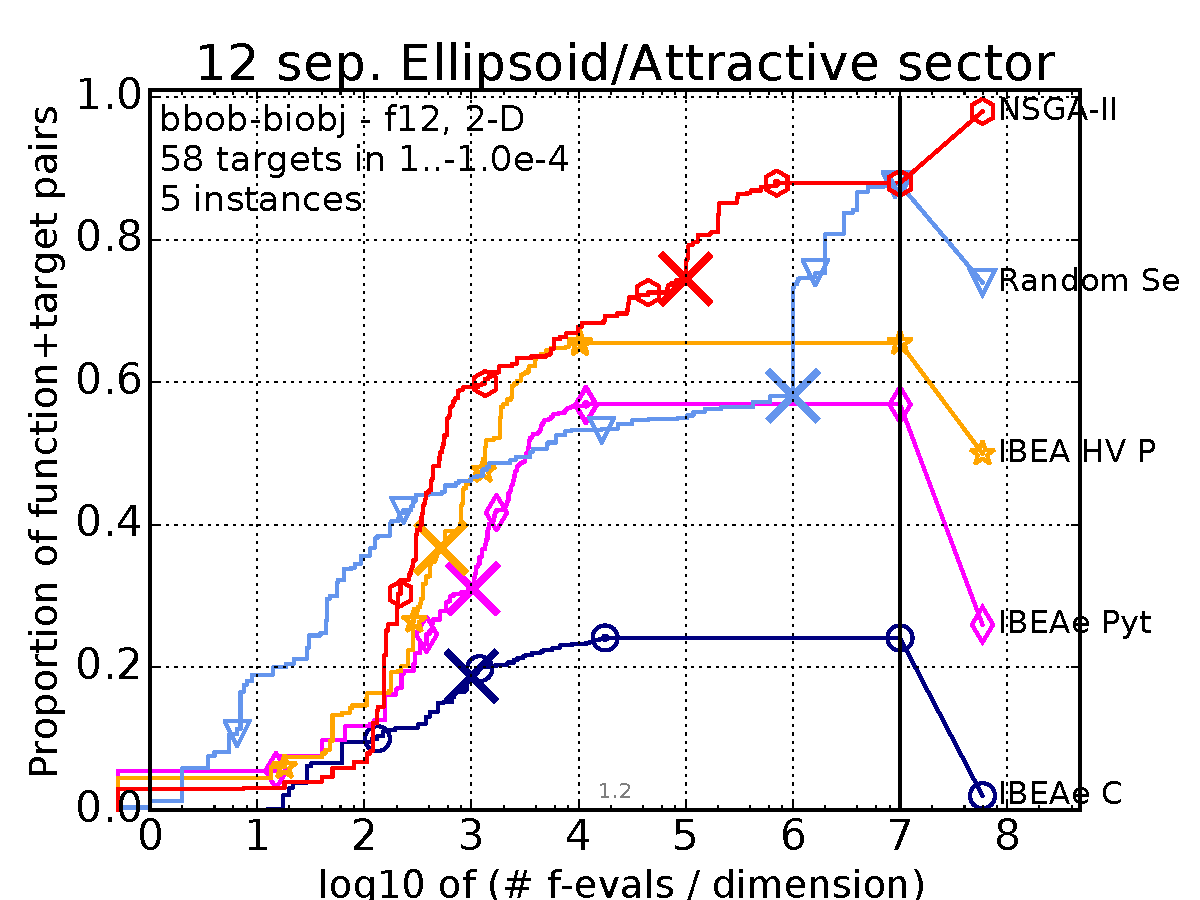
\includegraphics[width=0.2\textwidth]{pprldmany-single-functions/pprldmany_f012_02D}&
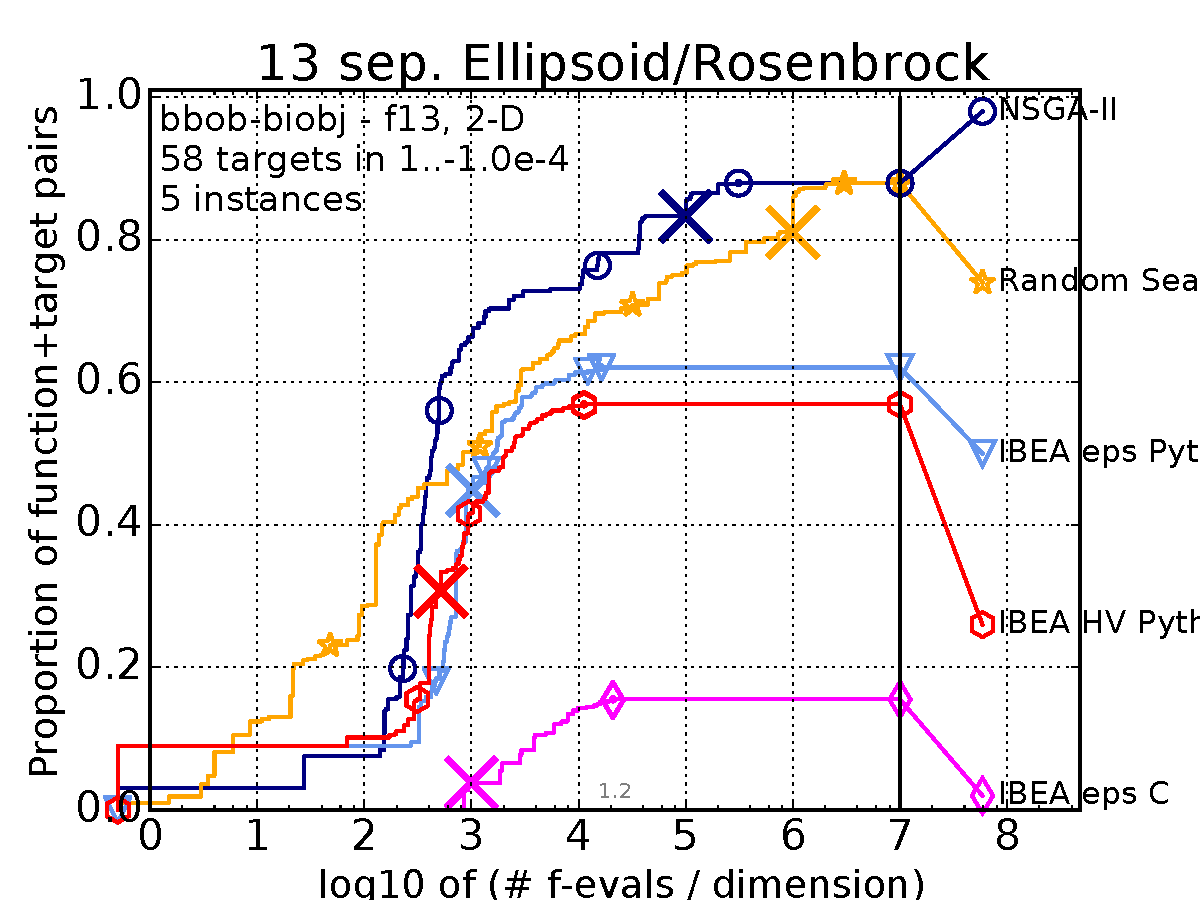
\includegraphics[width=0.2\textwidth]{pprldmany-single-functions/pprldmany_f013_02D}&
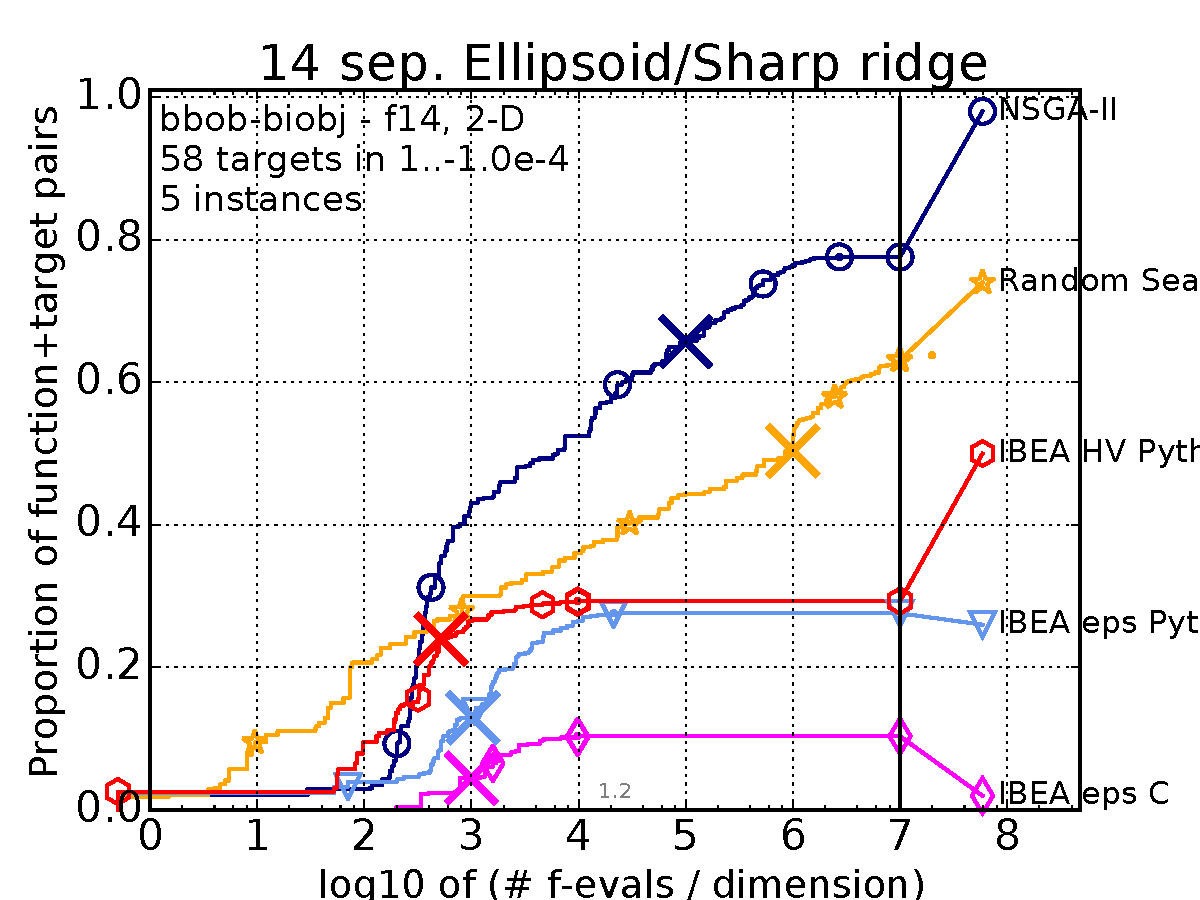
\includegraphics[width=0.2\textwidth]{pprldmany-single-functions/pprldmany_f014_02D}&
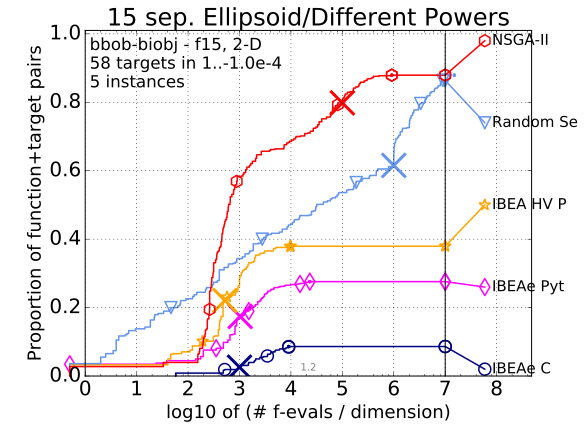
\includegraphics[width=0.2\textwidth]{pprldmany-single-functions/pprldmany_f015_02D}\\[-1.8ex]
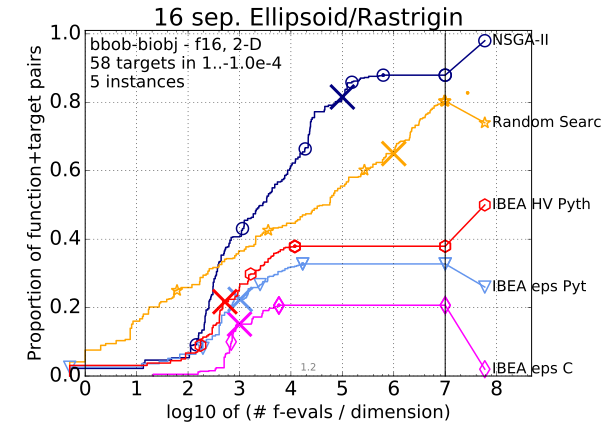
\includegraphics[width=0.2\textwidth]{pprldmany-single-functions/pprldmany_f016_02D}&
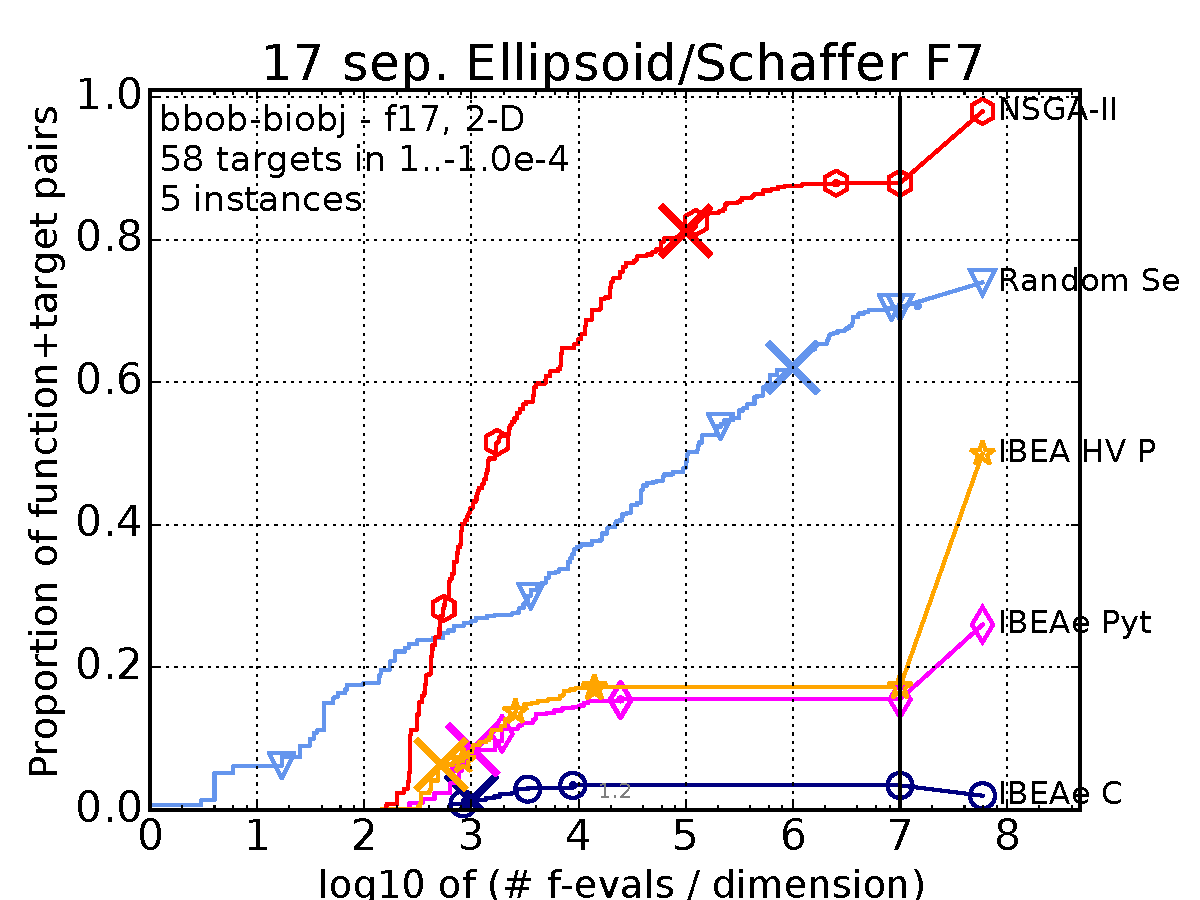
\includegraphics[width=0.2\textwidth]{pprldmany-single-functions/pprldmany_f017_02D}&
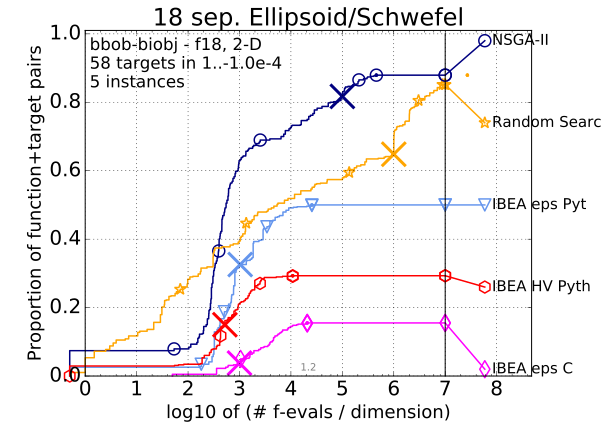
\includegraphics[width=0.2\textwidth]{pprldmany-single-functions/pprldmany_f018_02D}&
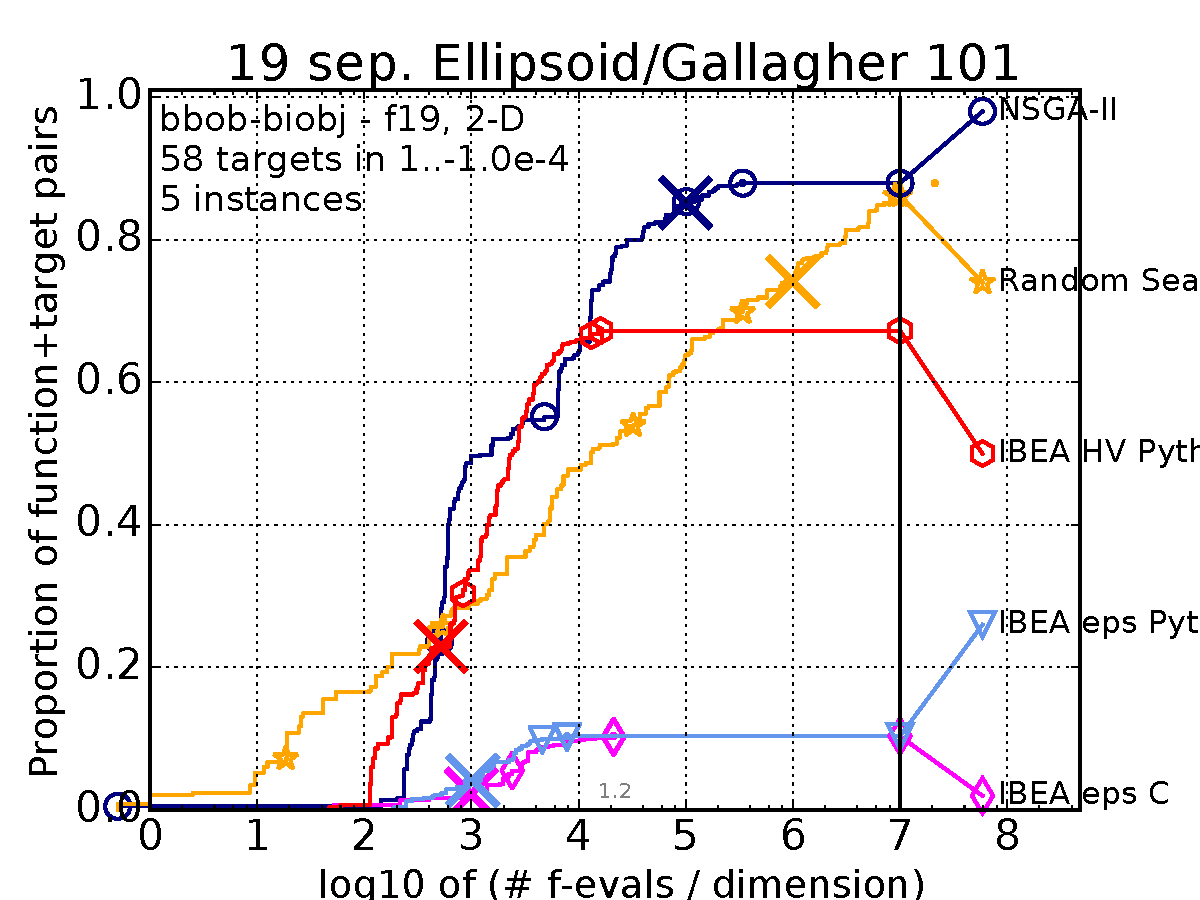
\includegraphics[width=0.2\textwidth]{pprldmany-single-functions/pprldmany_f019_02D}&
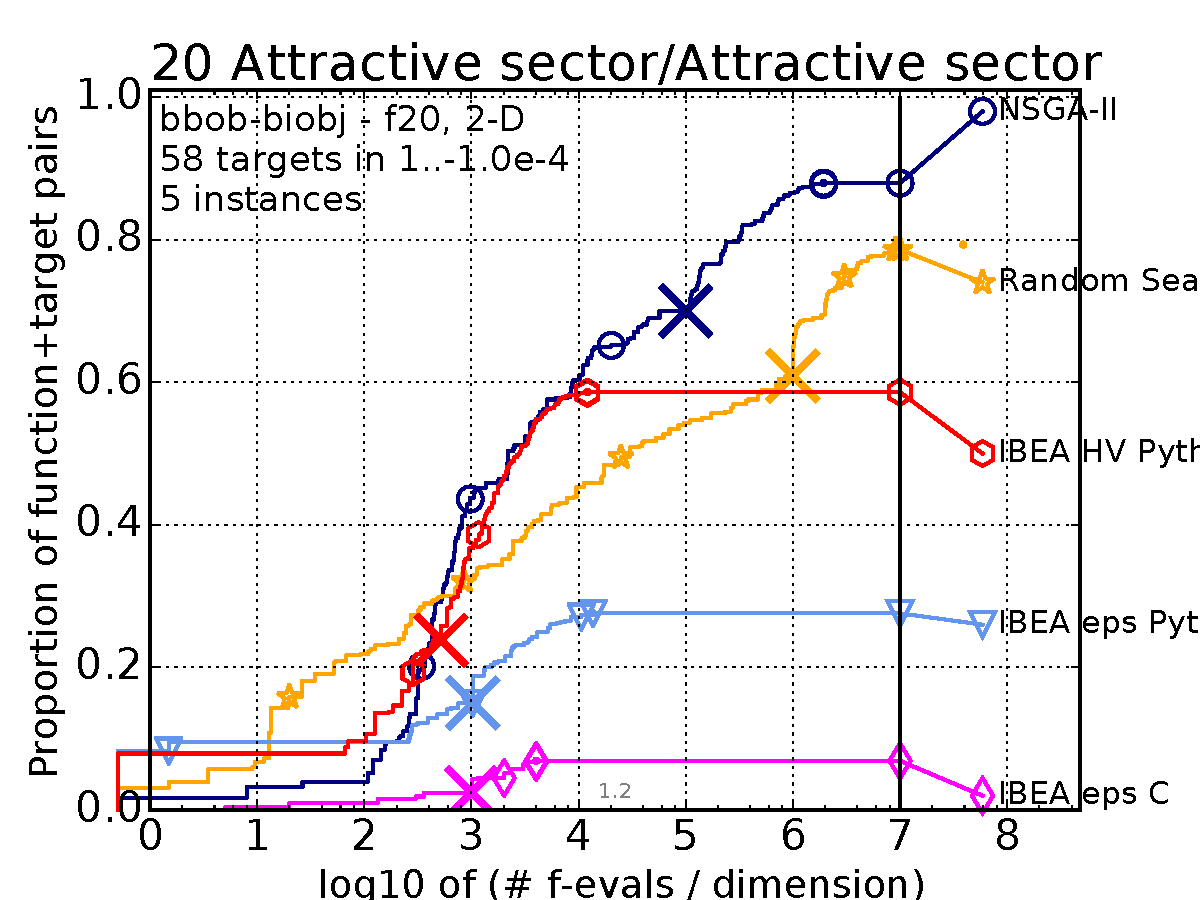
\includegraphics[width=0.2\textwidth]{pprldmany-single-functions/pprldmany_f020_02D}\\[-1.8ex]
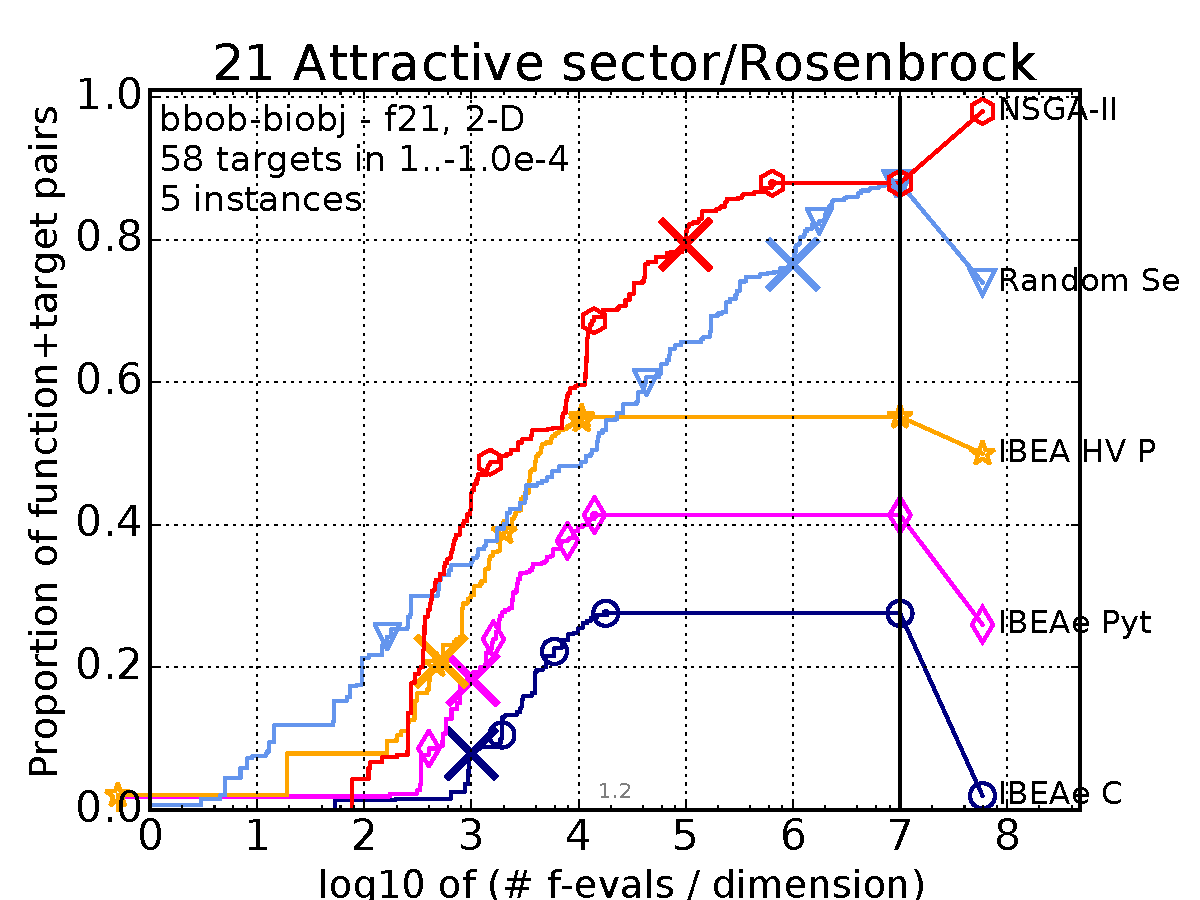
\includegraphics[width=0.2\textwidth]{pprldmany-single-functions/pprldmany_f021_02D}&
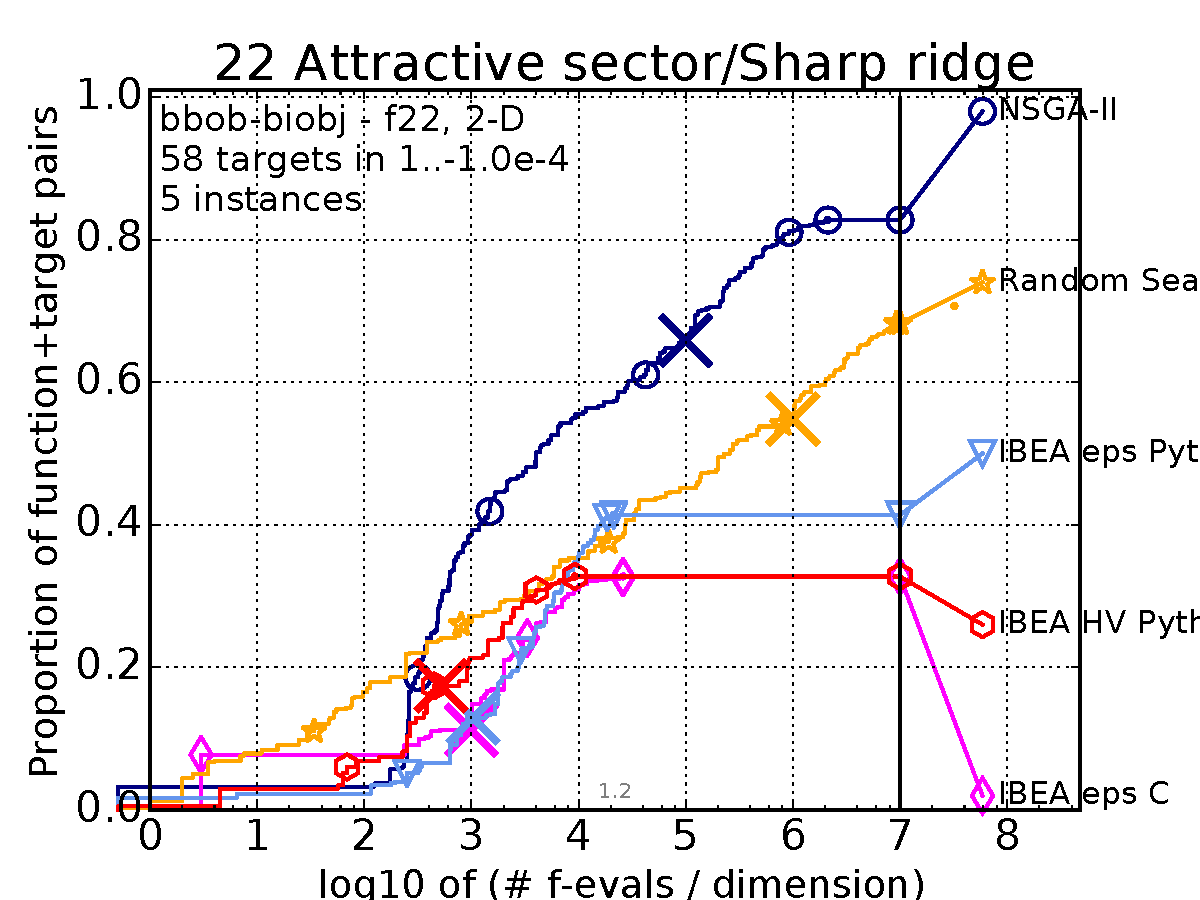
\includegraphics[width=0.2\textwidth]{pprldmany-single-functions/pprldmany_f022_02D}&
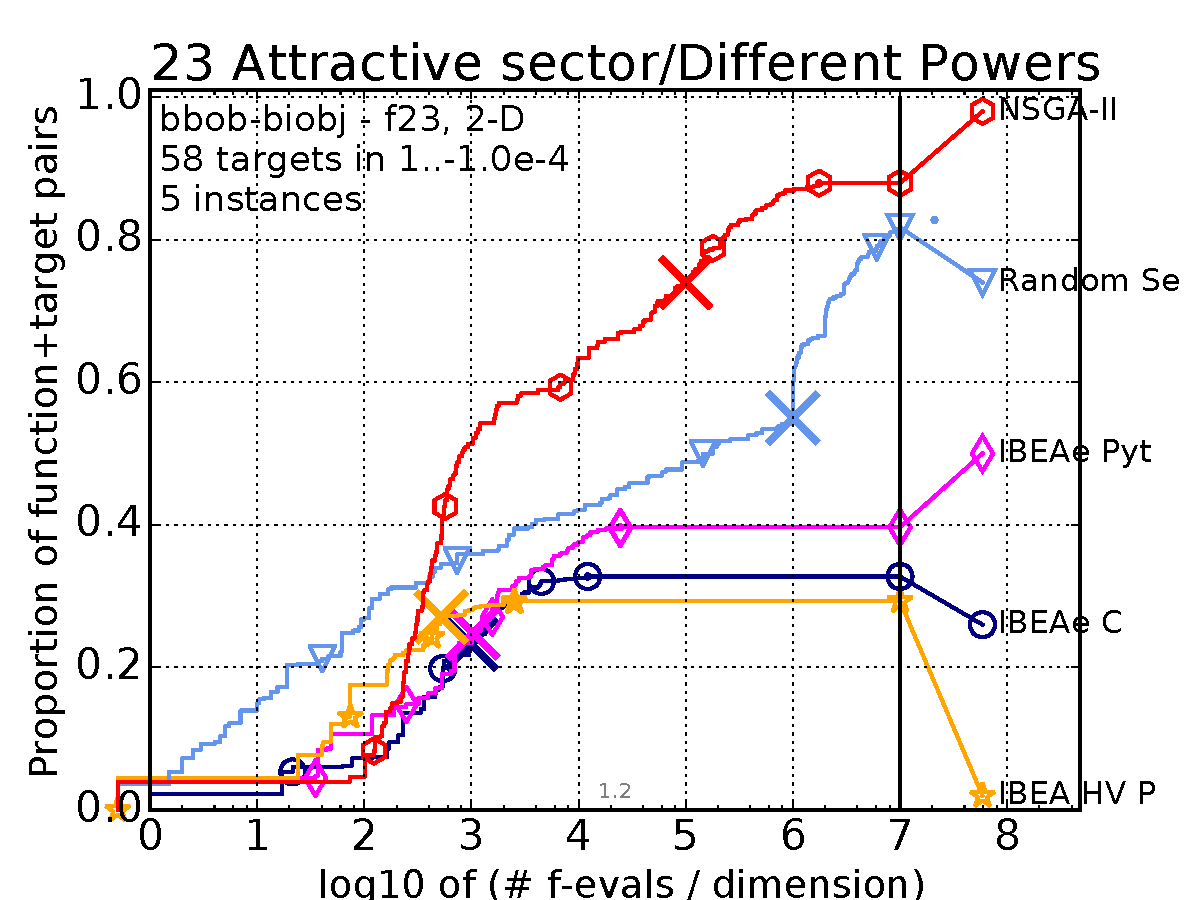
\includegraphics[width=0.2\textwidth]{pprldmany-single-functions/pprldmany_f023_02D}&
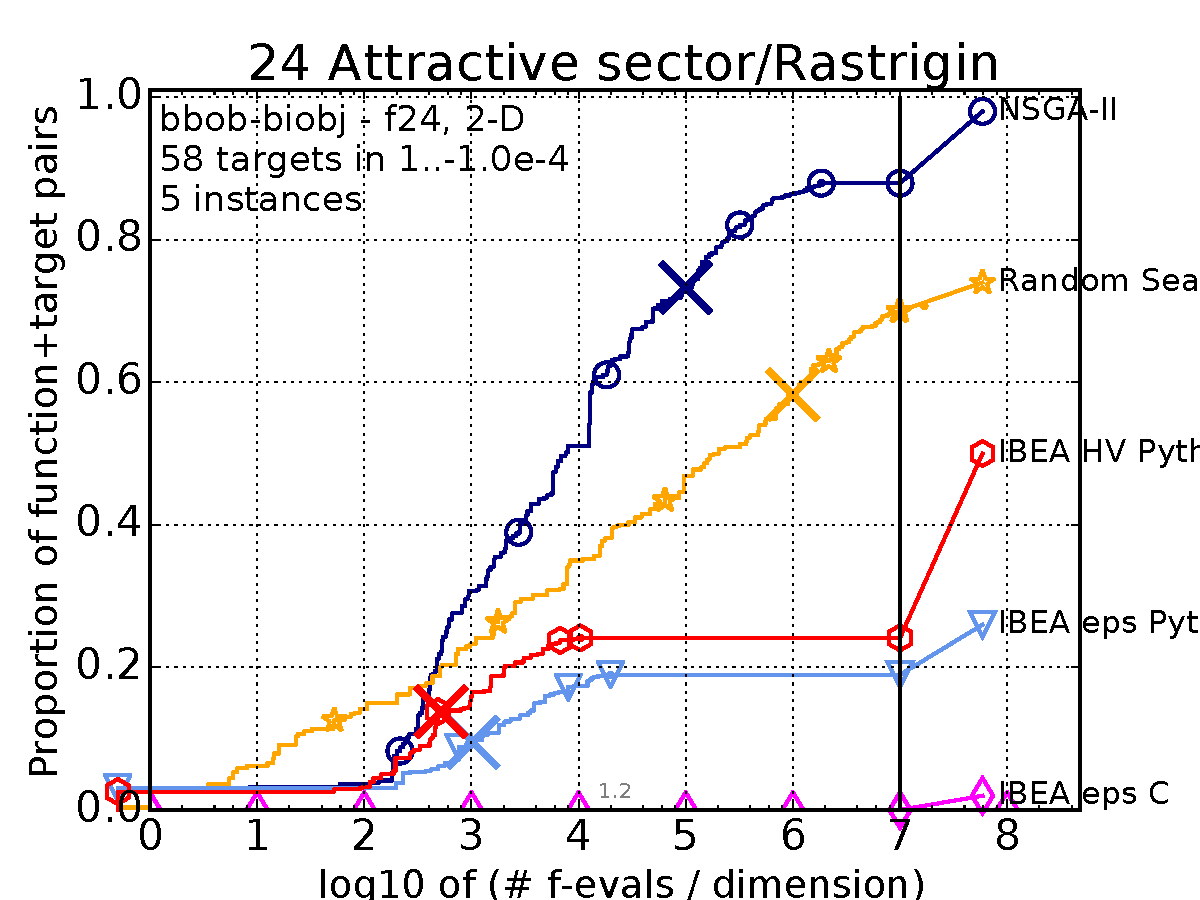
\includegraphics[width=0.2\textwidth]{pprldmany-single-functions/pprldmany_f024_02D}&
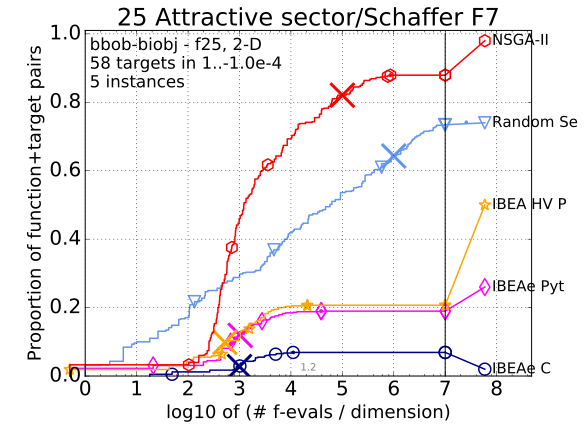
\includegraphics[width=0.2\textwidth]{pprldmany-single-functions/pprldmany_f025_02D}\\[-1.8ex]
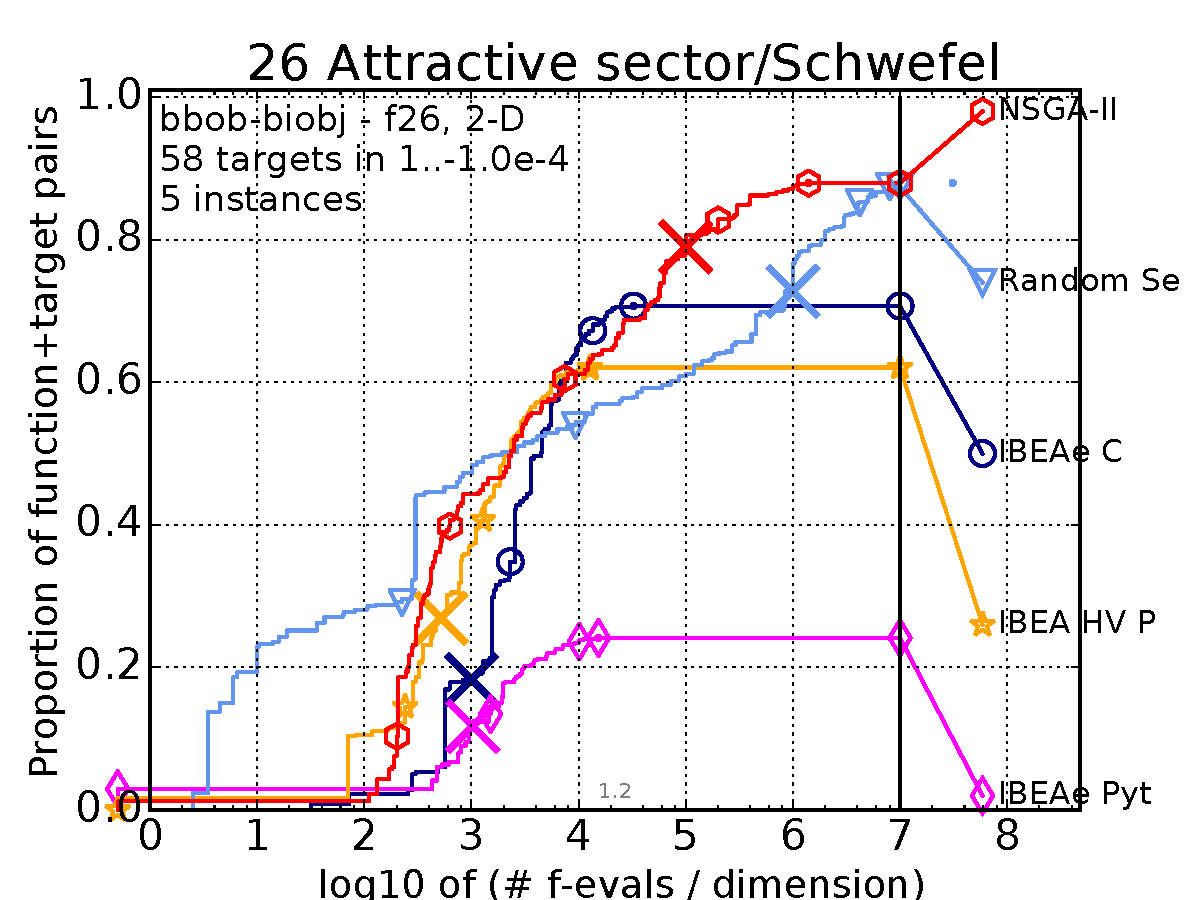
\includegraphics[width=0.2\textwidth]{pprldmany-single-functions/pprldmany_f026_02D}&
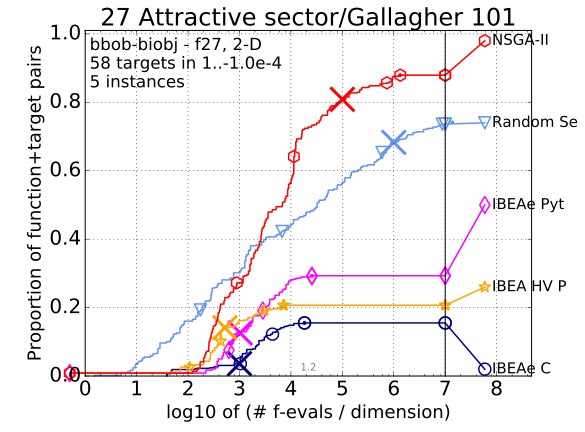
\includegraphics[width=0.2\textwidth]{pprldmany-single-functions/pprldmany_f027_02D}&
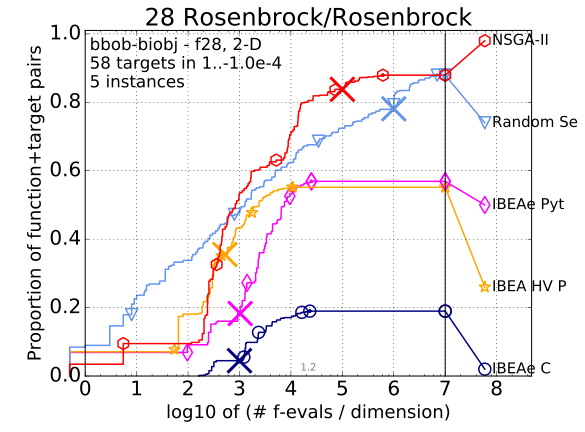
\includegraphics[width=0.2\textwidth]{pprldmany-single-functions/pprldmany_f028_02D}&
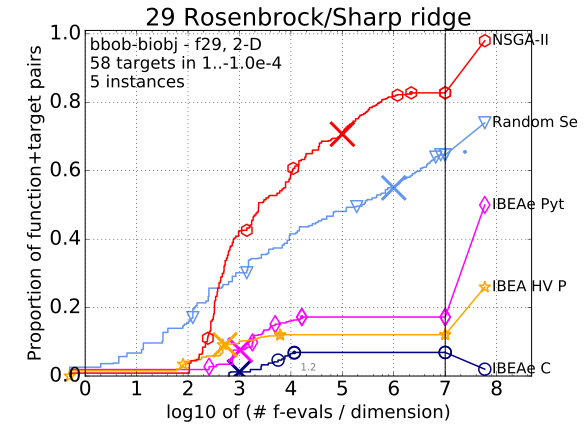
\includegraphics[width=0.2\textwidth]{pprldmany-single-functions/pprldmany_f029_02D}&
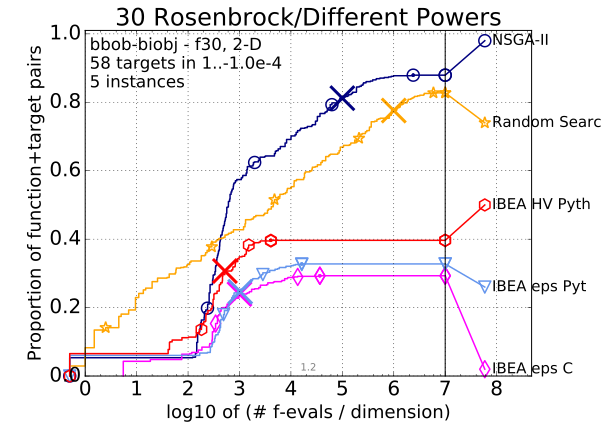
\includegraphics[width=0.2\textwidth]{pprldmany-single-functions/pprldmany_f030_02D}\\[-1.8ex]
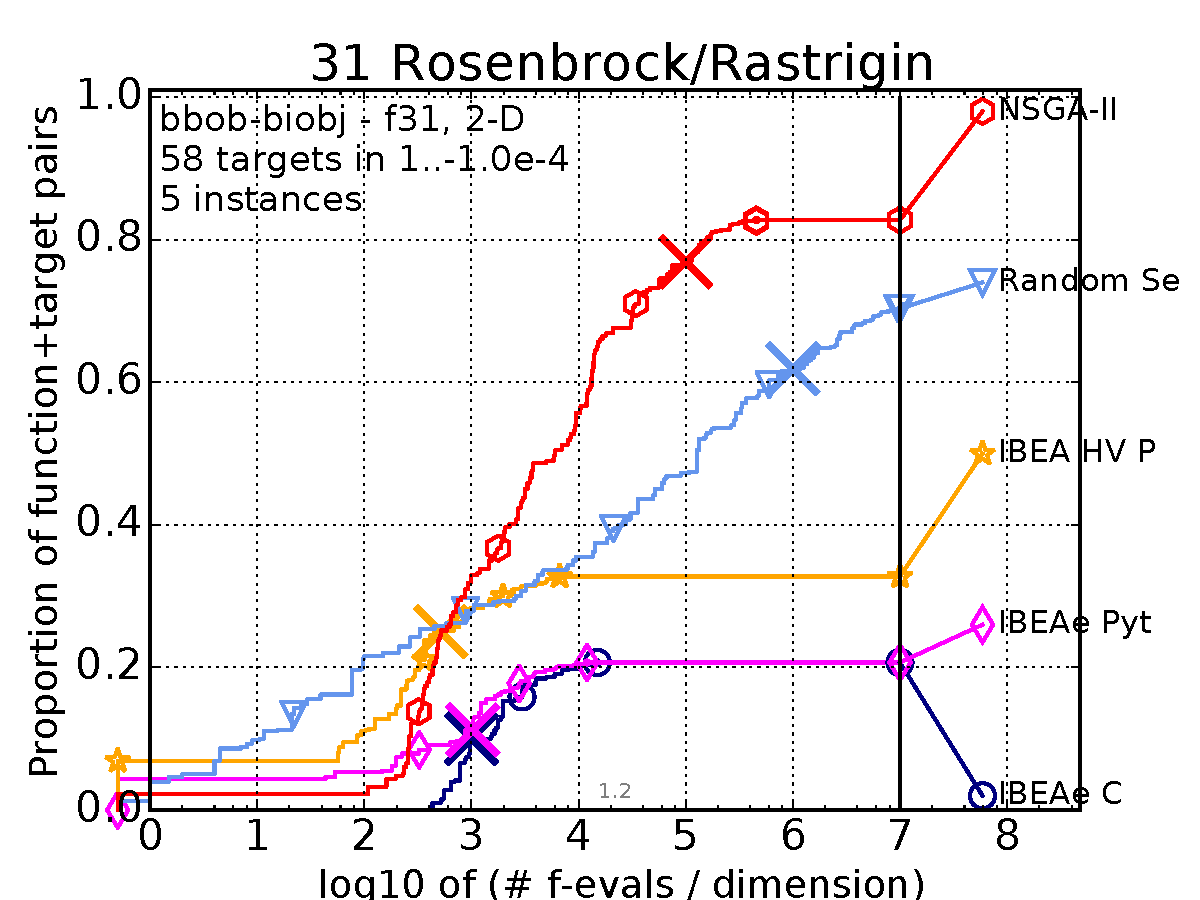
\includegraphics[width=0.2\textwidth]{pprldmany-single-functions/pprldmany_f031_02D}&
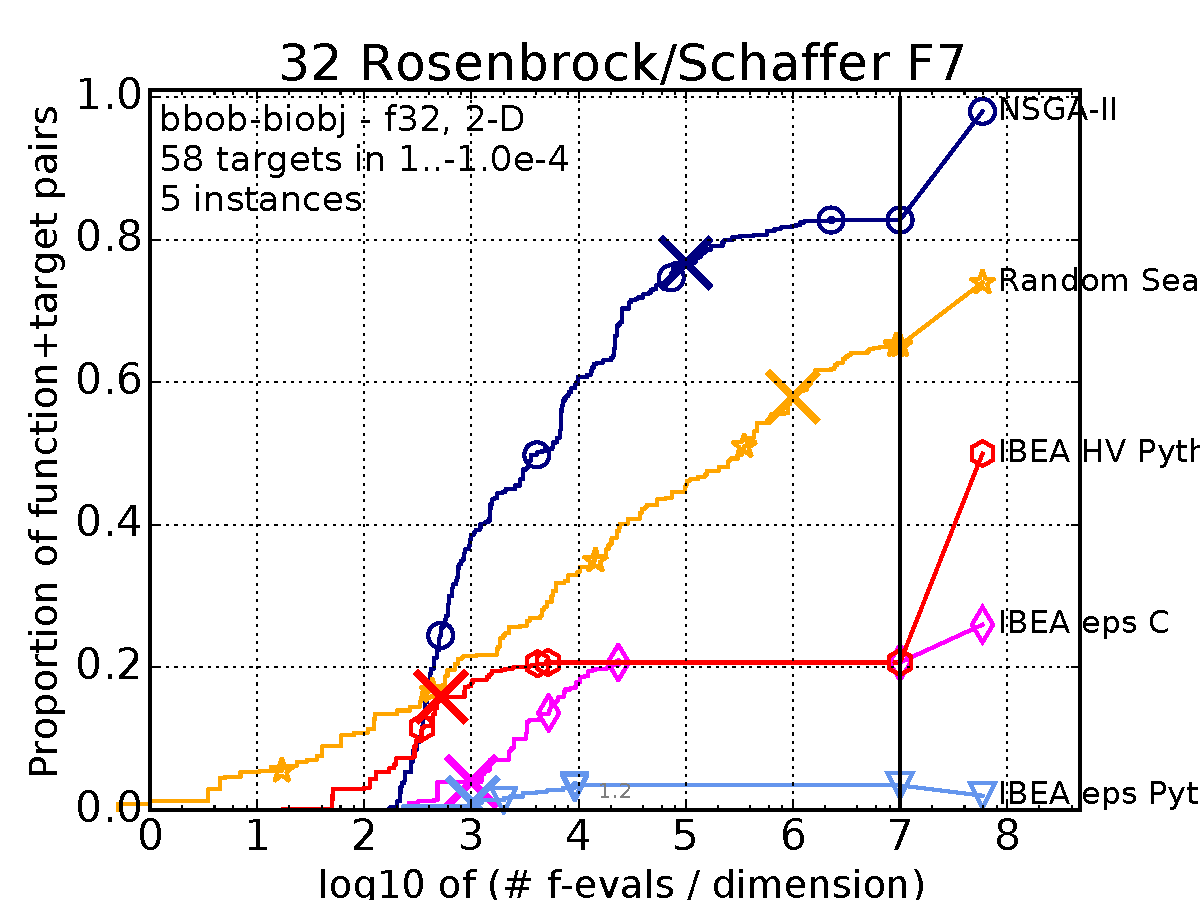
\includegraphics[width=0.2\textwidth]{pprldmany-single-functions/pprldmany_f032_02D}&
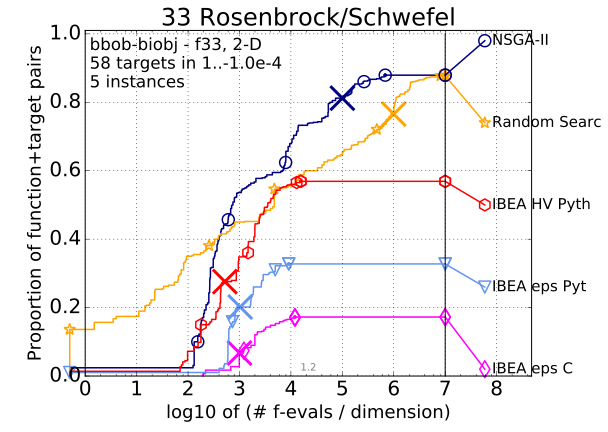
\includegraphics[width=0.2\textwidth]{pprldmany-single-functions/pprldmany_f033_02D}&
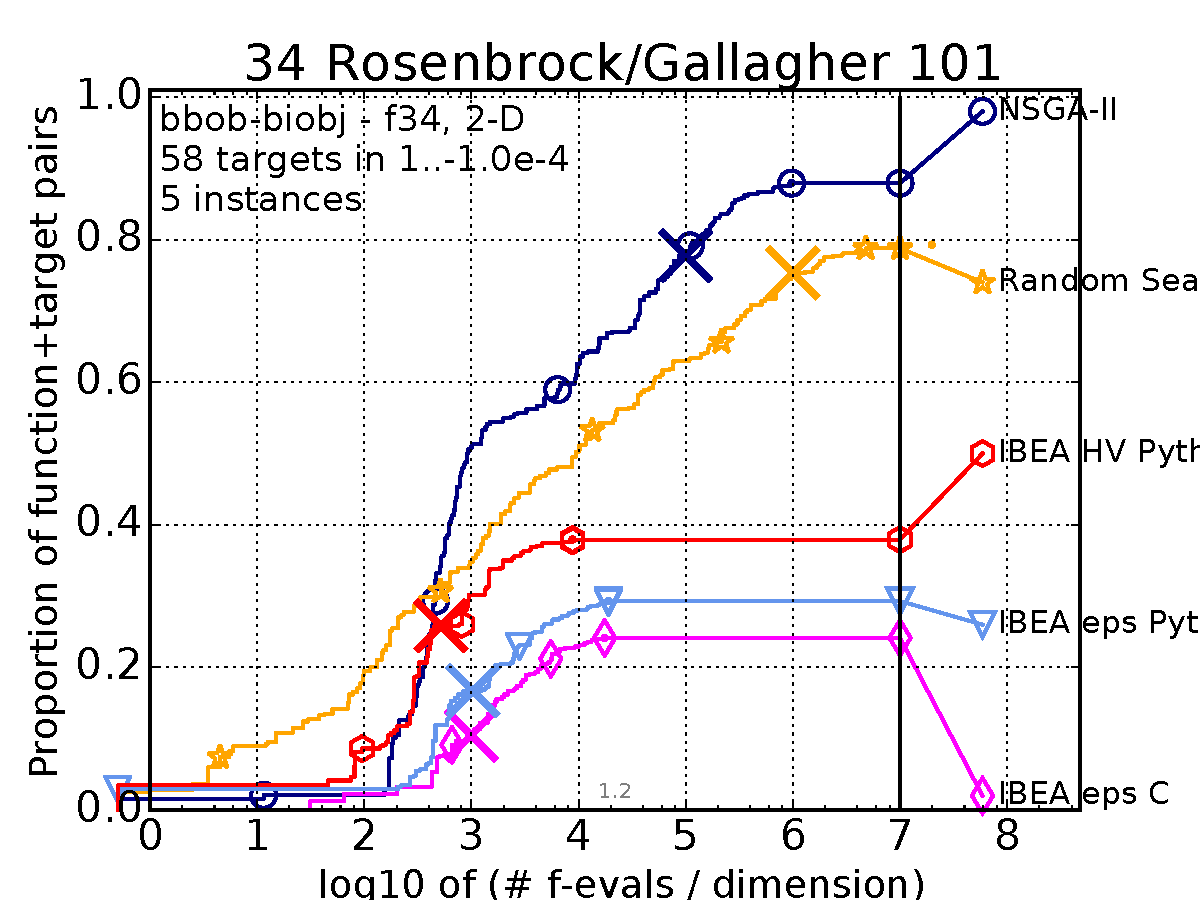
\includegraphics[width=0.2\textwidth]{pprldmany-single-functions/pprldmany_f034_02D}&
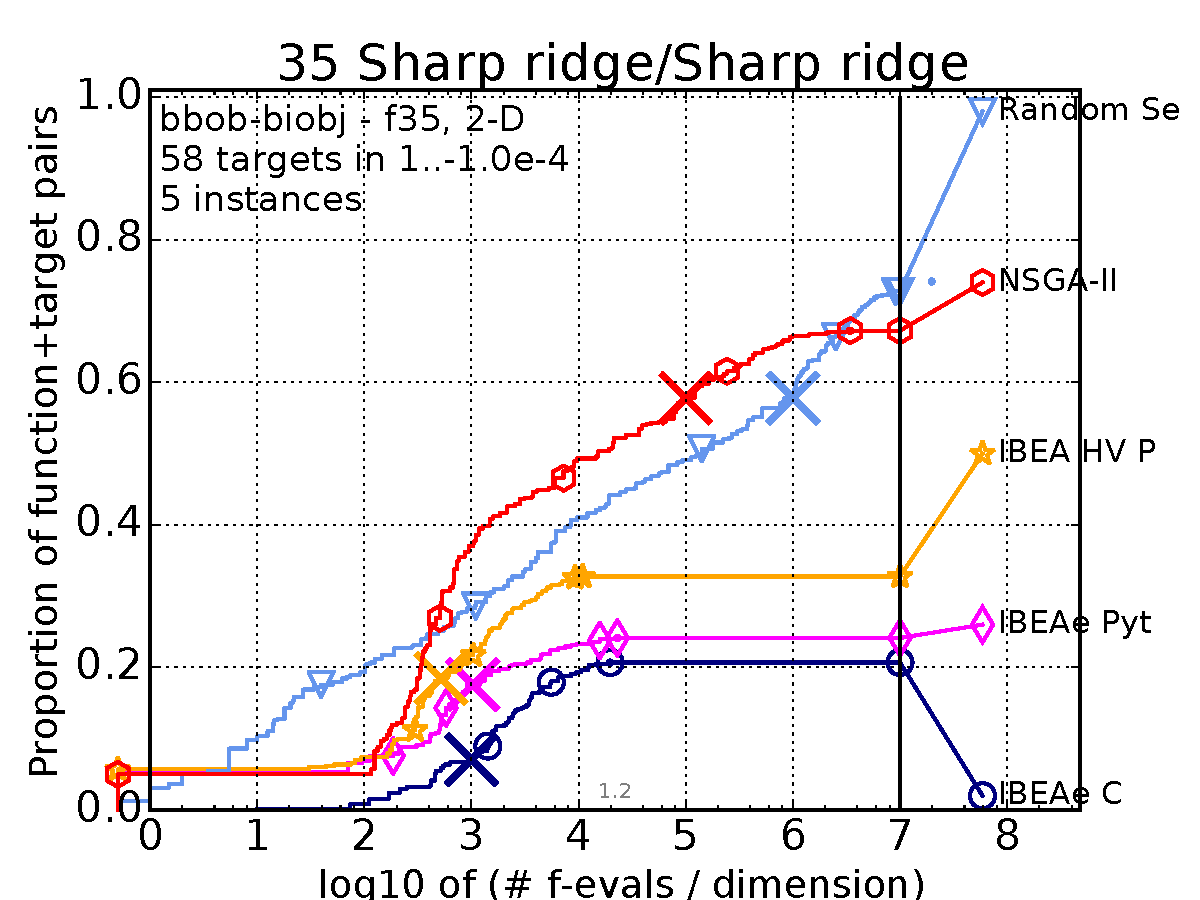
\includegraphics[width=0.2\textwidth]{pprldmany-single-functions/pprldmany_f035_02D}\\[-1.8ex]
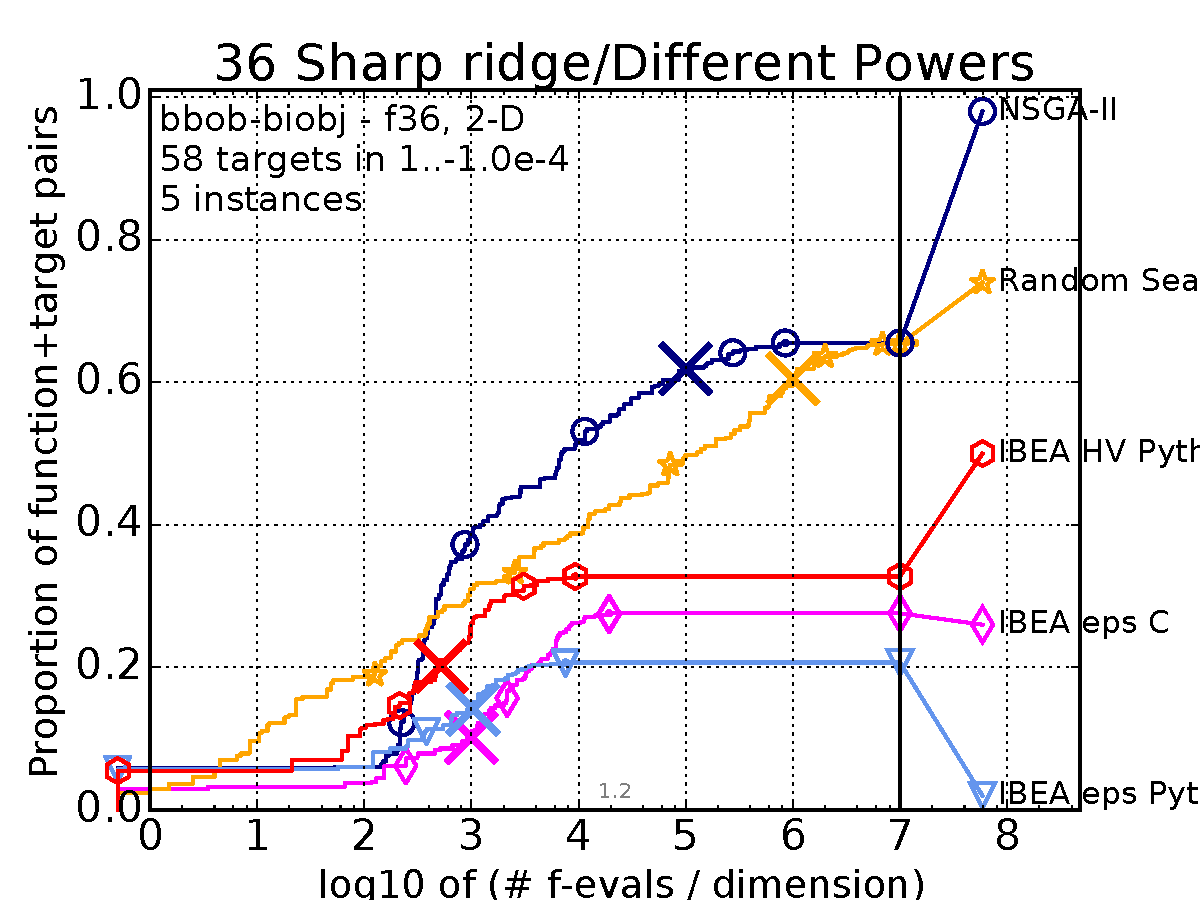
\includegraphics[width=0.2\textwidth]{pprldmany-single-functions/pprldmany_f036_02D}&
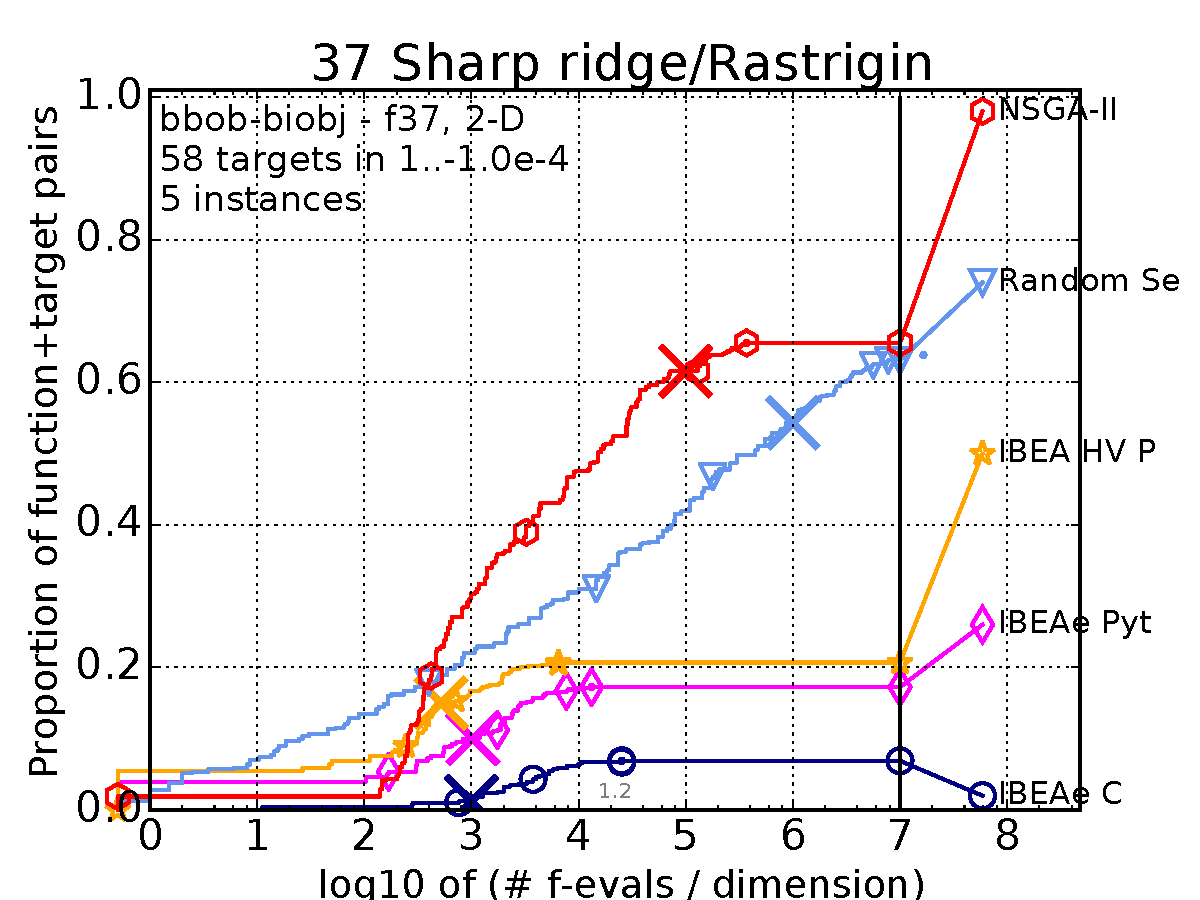
\includegraphics[width=0.2\textwidth]{pprldmany-single-functions/pprldmany_f037_02D}&
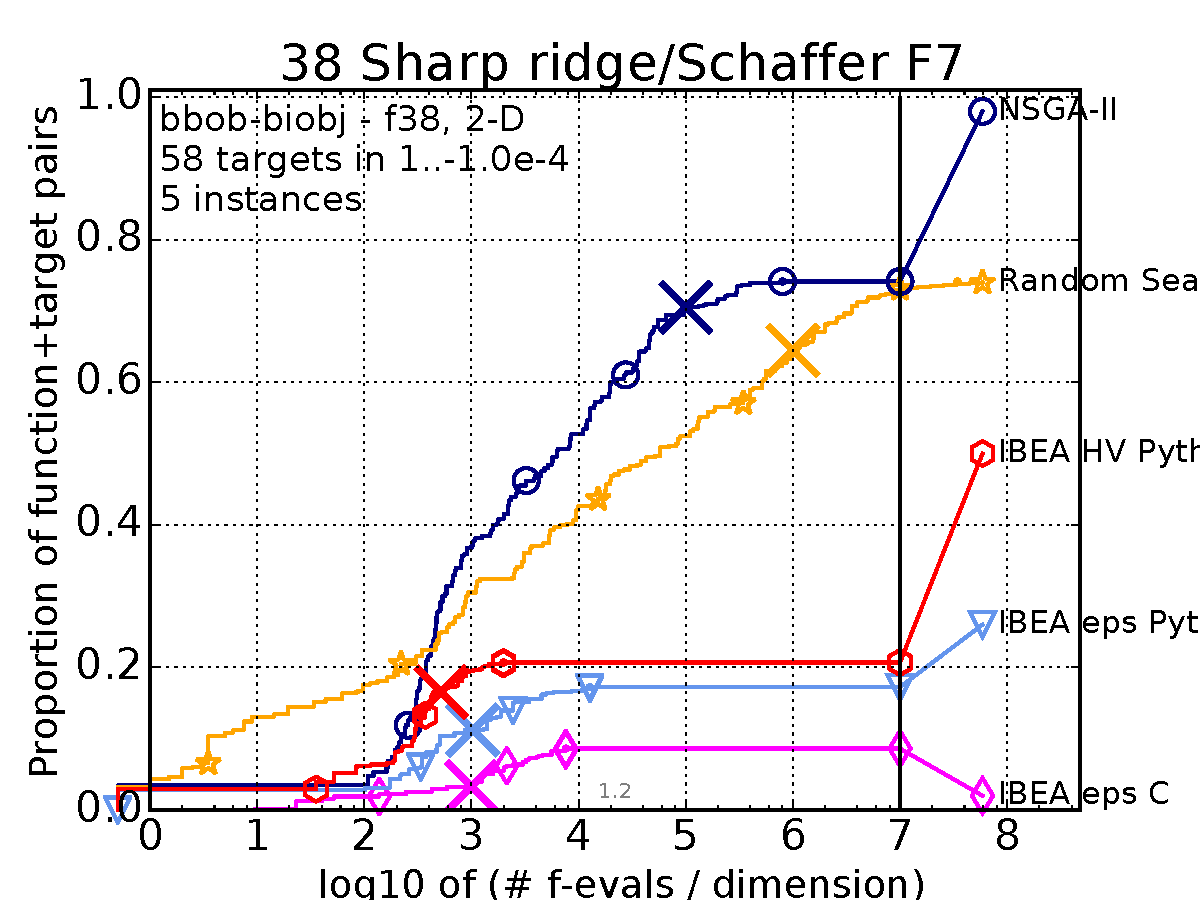
\includegraphics[width=0.2\textwidth]{pprldmany-single-functions/pprldmany_f038_02D}&
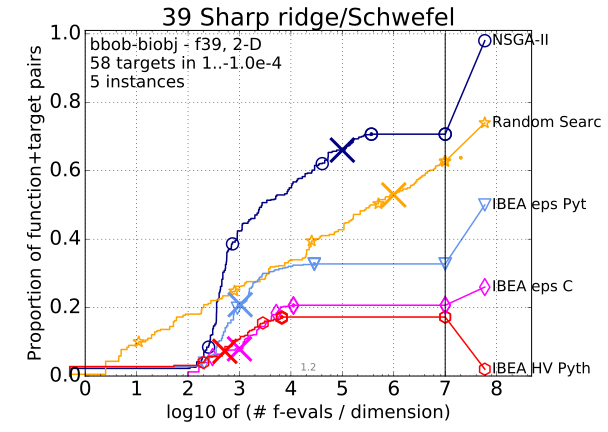
\includegraphics[width=0.2\textwidth]{pprldmany-single-functions/pprldmany_f039_02D}&
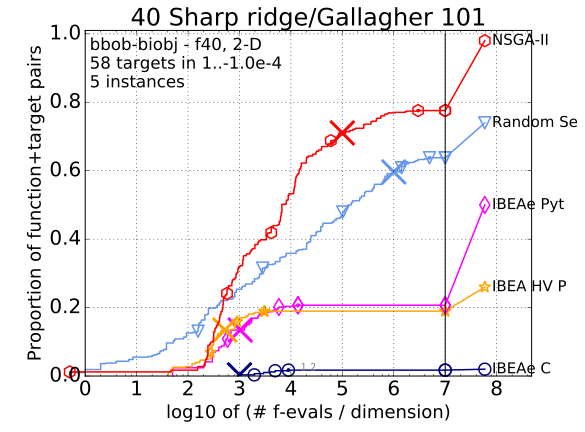
\includegraphics[width=0.2\textwidth]{pprldmany-single-functions/pprldmany_f040_02D}\\[-1.8ex]

\end{tabular}
 \caption{\label{fig:ECDFsingleOne}
 Bootstrapped empirical cumulative distribution of the number of objective function evaluations divided by dimension (FEvals/DIM) for $58$ targets with target precision in $\{-10^{-4}, -10^{-4.2}, $ $-10^{-4.4}, -10^{-4.6}, -10^{-4.8}, -10^{-5}, 0, 10^{-5}, 10^{-4.9}, 10^{-4.8}, \dots, 10^{-0.1}, 10^0\}$ for each single function $f_{1}$ to $f_{40}$ in 10-D. 
}
\end{figure*}

\begin{figure*}
\centering
\begin{tabular}{@{\hspace*{-0.005\textwidth}}l@{\hspace*{-0.005\textwidth}}l@{\hspace*{-0.005\textwidth}}l@{\hspace*{-0.005\textwidth}}l@{\hspace*{-0.005\textwidth}}l@{\hspace*{-0.005\textwidth}}}
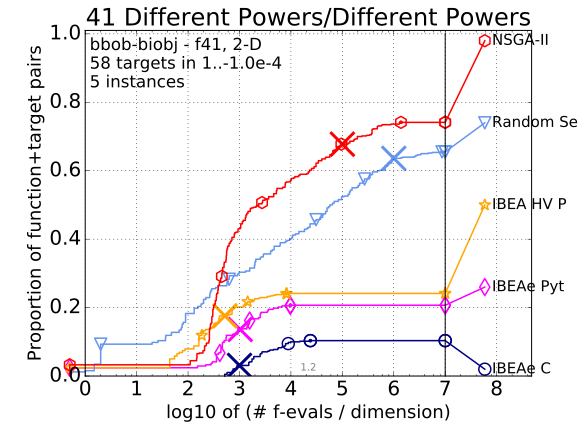
\includegraphics[width=0.2\textwidth]{pprldmany-single-functions/pprldmany_f041_02D}&
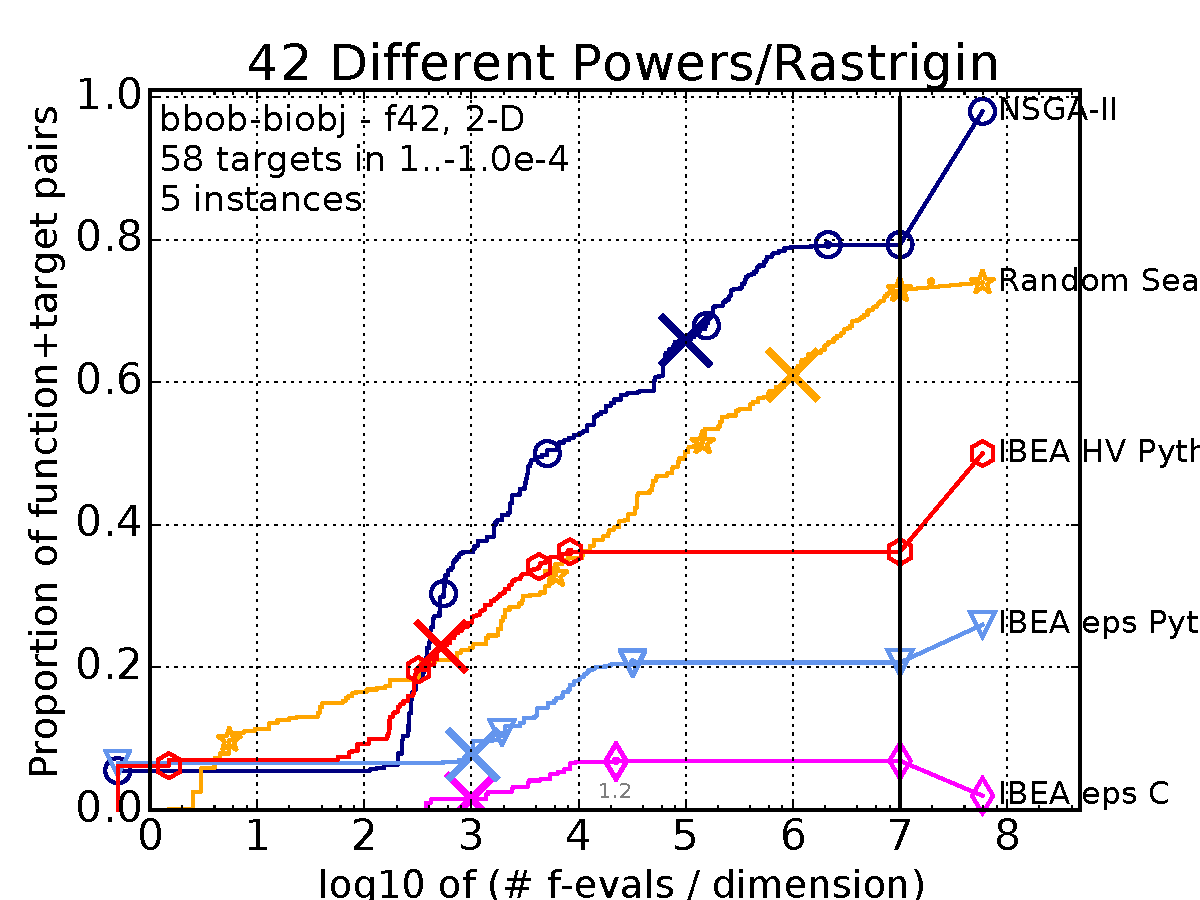
\includegraphics[width=0.2\textwidth]{pprldmany-single-functions/pprldmany_f042_02D}&
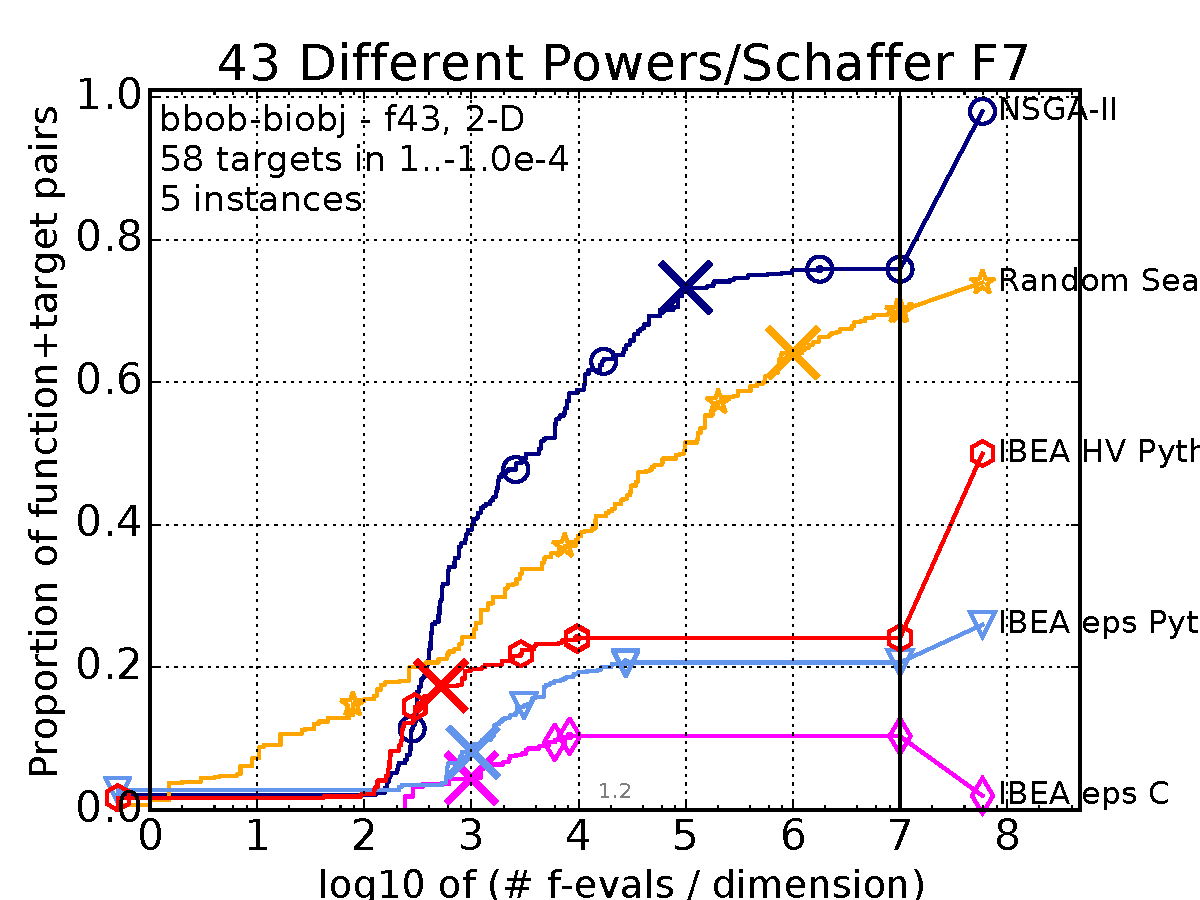
\includegraphics[width=0.2\textwidth]{pprldmany-single-functions/pprldmany_f043_02D}&
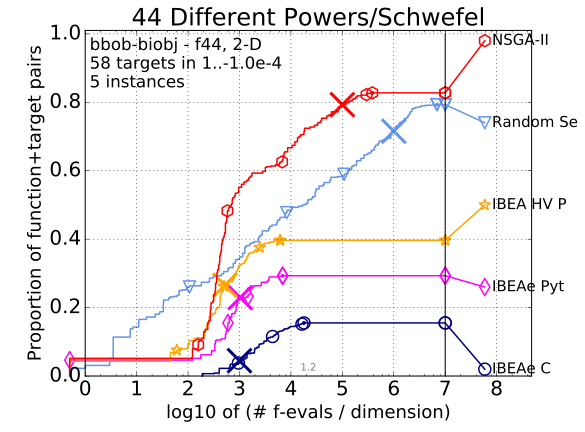
\includegraphics[width=0.2\textwidth]{pprldmany-single-functions/pprldmany_f044_02D}&
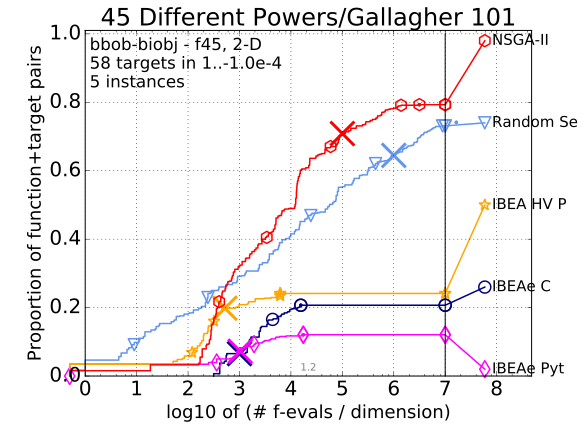
\includegraphics[width=0.2\textwidth]{pprldmany-single-functions/pprldmany_f045_02D}\\[-1.8ex]
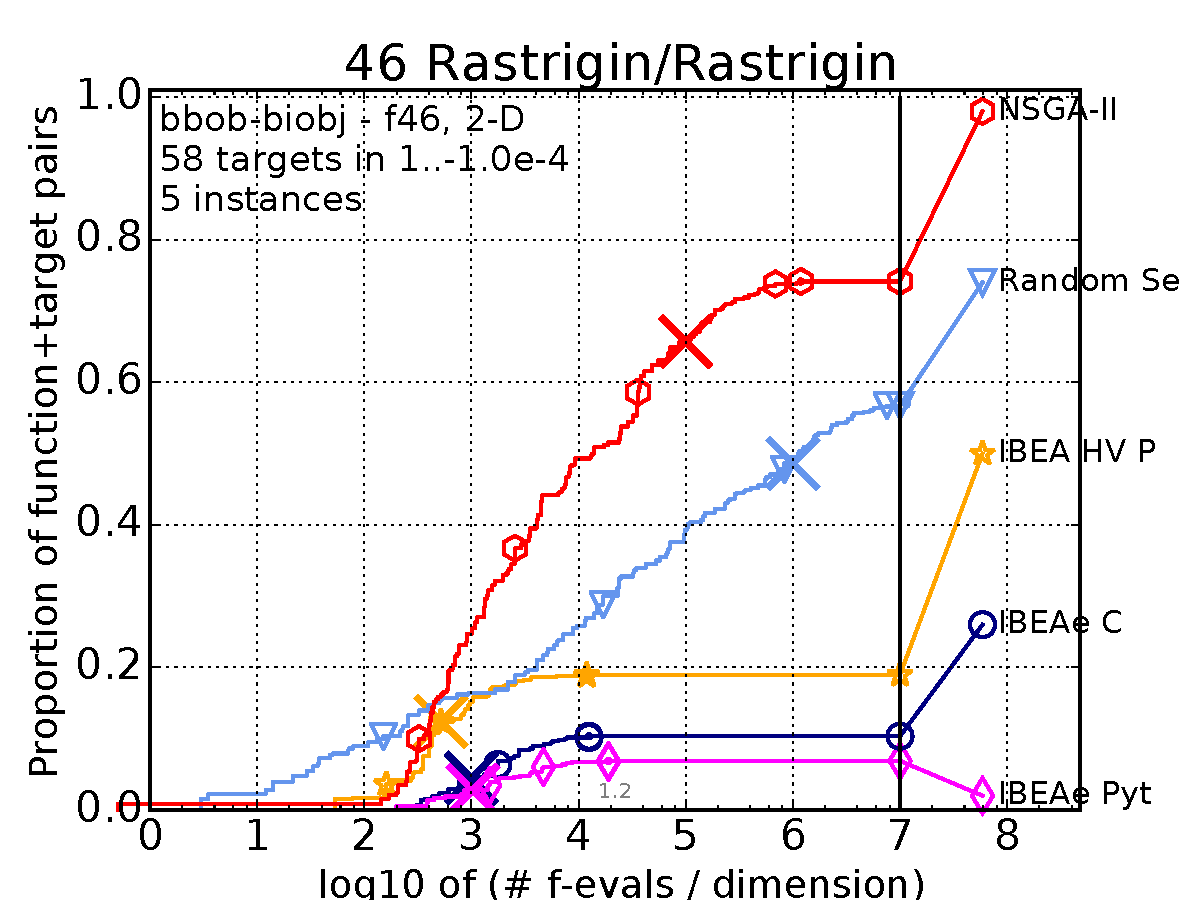
\includegraphics[width=0.2\textwidth]{pprldmany-single-functions/pprldmany_f046_02D}&
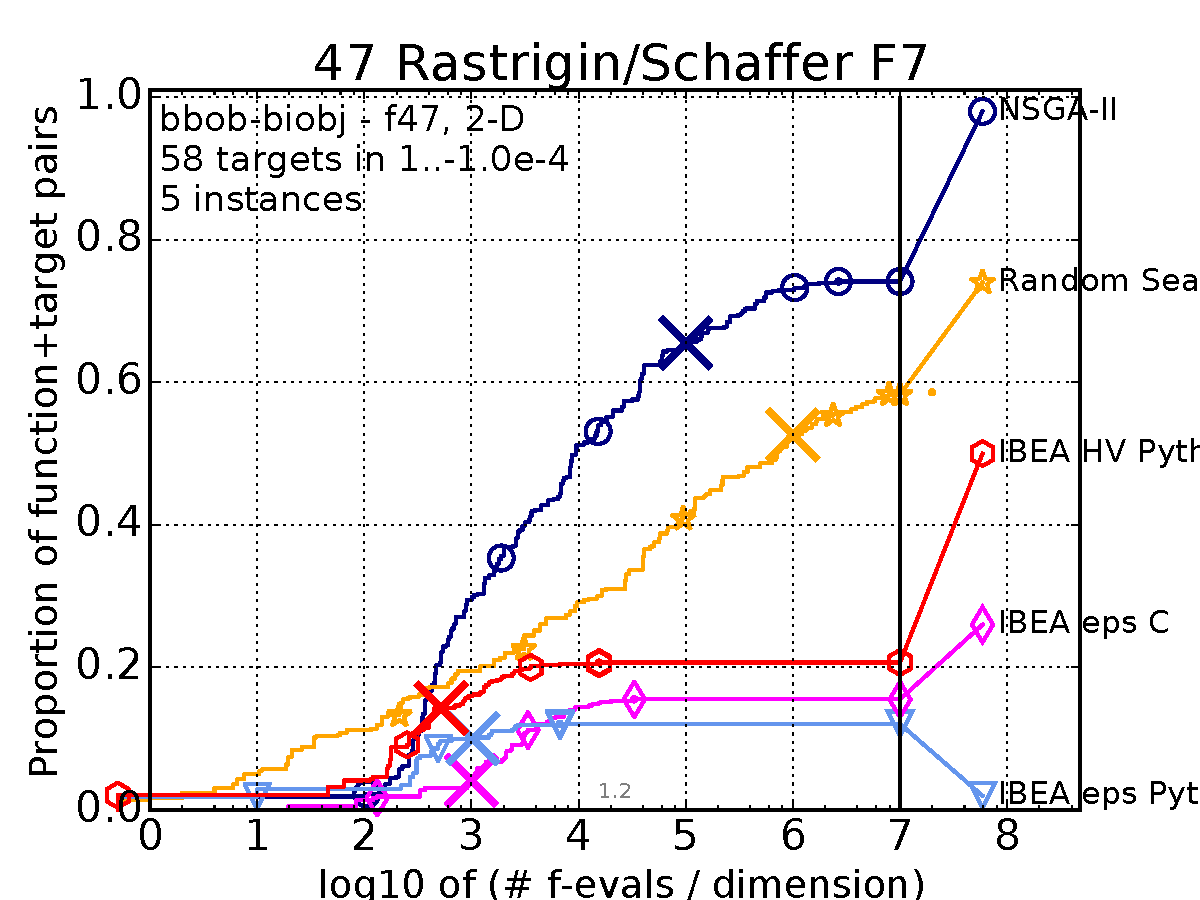
\includegraphics[width=0.2\textwidth]{pprldmany-single-functions/pprldmany_f047_02D}&
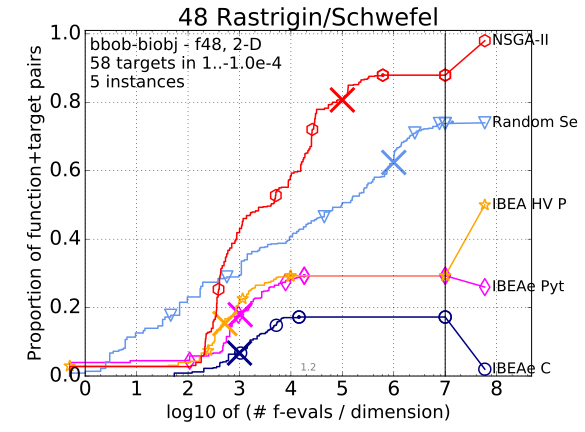
\includegraphics[width=0.2\textwidth]{pprldmany-single-functions/pprldmany_f048_02D}&
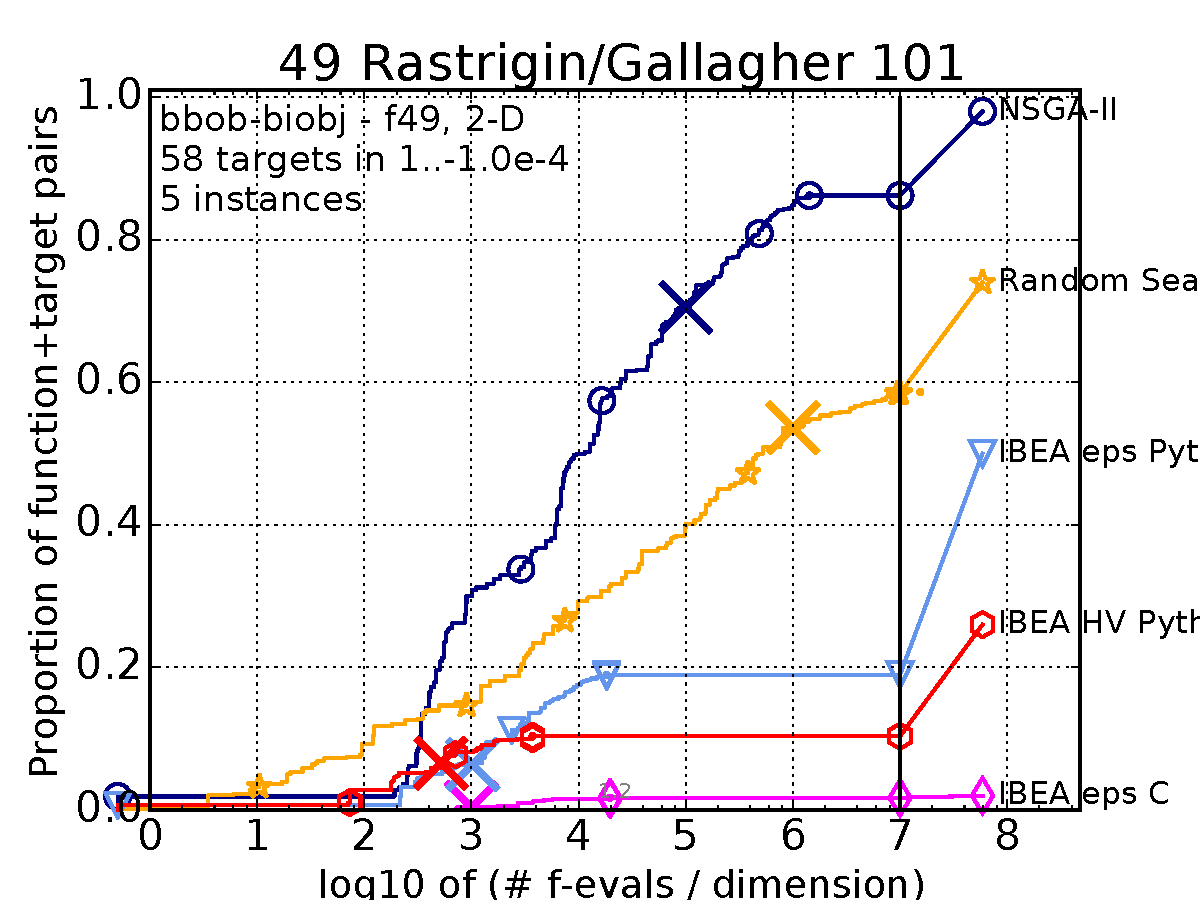
\includegraphics[width=0.2\textwidth]{pprldmany-single-functions/pprldmany_f049_02D}&
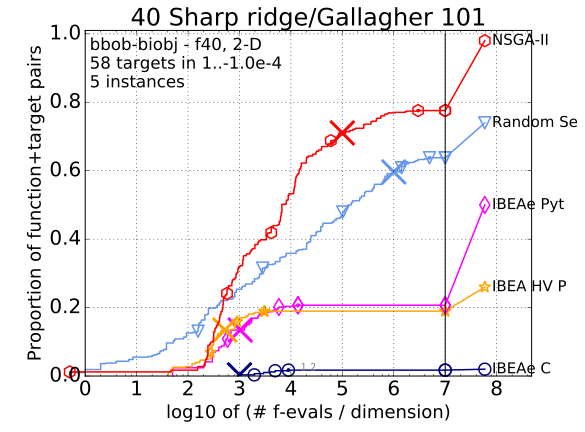
\includegraphics[width=0.2\textwidth]{pprldmany-single-functions/pprldmany_f040_02D}\\[-1.8ex]
\includegraphics[width=0.2\textwidth]{pprldmany-single-functions/pprldmany_f051_02D}&
\includegraphics[width=0.2\textwidth]{pprldmany-single-functions/pprldmany_f052_02D}&
\includegraphics[width=0.2\textwidth]{pprldmany-single-functions/pprldmany_f053_02D}&
\includegraphics[width=0.2\textwidth]{pprldmany-single-functions/pprldmany_f054_02D}&
\includegraphics[width=0.2\textwidth]{pprldmany-single-functions/pprldmany_f055_02D}\\[-1.8ex]
\end{tabular}
 \caption{\label{fig:ECDFsingleTwo}
 Bootstrapped empirical cumulative distribution of the number of objective function evaluations divided by dimension (FEvals/DIM) as in Fig.~\ref{fig:ECDFsingleOne} but for functions $f_{41}$ to $f_{55}$ in 10-D.
}
\end{figure*}




%%%%%%%%%%%%%%%%%%%%%%%%%%%%%%%%%%%%%%%%%%%%%%%%%%%%%%%%%%%%%%%%%%%%%%%%%%%%%%%
%%%%%%%%%%%%%%%%%%%%%%%%%%%%%%%%%%%%%%%%%%%%%%%%%%%%%%%%%%%%%%%%%%%%%%%%%%%%%%%

% Empirical cumulative distribution functions (ECDFs) per function group (5-D)

%%%%%%%%%%%%%%%%%%%%%%%%%%%%%%%%%%%%%%%%%%%%%%%%%%%%%%%%%%%%%%%%%%%%%%%%%%%%%%%

\begin{figure*}
\begin{tabular}{@{\hspace*{-0.009\textwidth}}c@{\hspace*{-0.014\textwidth}}c@{\hspace*{-0.016\textwidth}}c@{\hspace*{-0.02\textwidth}}c}
separable-separable & separable-moderate & separable-ill-cond. & separable-multimodal\\
\includegraphics[width=0.268\textwidth,trim=0 0 0 13mm, clip]{pprldmany_02D_1-separable_1-separable} &
\includegraphics[width=0.268\textwidth,trim=0 0 0 13mm, clip]{pprldmany_02D_1-separable_2-moderate} &
\includegraphics[width=0.268\textwidth,trim=0 0 0 13mm, clip]{pprldmany_02D_1-separable_3-ill-conditioned} &
\includegraphics[width=0.268\textwidth,trim=0 0 0 13mm, clip]{pprldmany_02D_1-separable_4-multi-modal}\\
separable-weakstructure & moderate-moderate & moderate-ill-cond. & moderate-multimodal\\
\includegraphics[width=0.268\textwidth,trim=0 0 0 13mm, clip]{pprldmany_02D_1-separable_5-weakly-structured} &
\includegraphics[width=0.268\textwidth,trim=0 0 0 13mm, clip]{pprldmany_02D_2-moderate_2-moderate} &
\includegraphics[width=0.268\textwidth,trim=0 0 0 13mm, clip]{pprldmany_02D_2-moderate_3-ill-conditioned} &
\includegraphics[width=0.268\textwidth,trim=0 0 0 13mm, clip]{pprldmany_02D_2-moderate_4-multi-modal}\\
moderate-weakstructure & ill-cond.-ill-cond. & ill-cond.-multimodal & ill-cond.-weakstructure\\
\includegraphics[width=0.268\textwidth,trim=0 0 0 13mm, clip]{pprldmany_02D_2-moderate_5-weakly-structured} &
\includegraphics[width=0.268\textwidth,trim=0 0 0 13mm, clip]{pprldmany_02D_3-ill-conditioned_3-ill-conditioned} &
\includegraphics[width=0.268\textwidth,trim=0 0 0 13mm, clip]{pprldmany_02D_3-ill-conditioned_4-multi-modal} &
\includegraphics[width=0.268\textwidth,trim=0 0 0 13mm, clip]{pprldmany_02D_3-ill-conditioned_5-weakly-structured} \\
multimodal-multimodal & multimodal-weakstructure & weakstructure-weakstructure & all 55 functions\\
\includegraphics[width=0.268\textwidth,trim=0 0 0 13mm, clip]{pprldmany_02D_4-multi-modal_4-multi-modal} &
\includegraphics[width=0.268\textwidth,trim=0 0 0 13mm, clip]{pprldmany_02D_4-multi-modal_5-weakly-structured} &
\includegraphics[width=0.268\textwidth,trim=0 0 0 13mm, clip]{pprldmany_02D_5-weakly-structured_5-weakly-structured} &
\includegraphics[width=0.268\textwidth,trim=0 0 0 13mm, clip]{pprldmany_02D_noiselessall}
\vspace*{-0.5ex}
\end{tabular}
 \caption{\label{fig:ECDFsGroupsFive}
 \bbobECDFslegend{4}
 }
\end{figure*}

%%%%%%%%%%%%%%%%%%%%%%%%%%%%%%%%%%%%%%%%%%%%%%%%%%%%%%%%%%%%%%%%%%%%%%%%%%%%%%%
%%%%%%%%%%%%%%%%%%%%%%%%%%%%%%%%%%%%%%%%%%%%%%%%%%%%%%%%%%%%%%%%%%%%%%%%%%%%%%%

% Empirical cumulative distribution functions (ECDFs) per function group (20-D)

%%%%%%%%%%%%%%%%%%%%%%%%%%%%%%%%%%%%%%%%%%%%%%%%%%%%%%%%%%%%%%%%%%%%%%%%%%%%%%%

%\begin{figure*}
%\begin{tabular}{@{\hspace*{-0.009\textwidth}}c@{\hspace*{-0.014\textwidth}}c@{\hspace*{-0.016\textwidth}}c@{\hspace*{-0.02\textwidth}}c}
%separable-separable & separable-moderate & separable-ill-cond. & separable-multimodal\\
%\includegraphics[width=0.268\textwidth,trim=0 0 0 13mm, clip]{pprldmany_20D_1-separable_1-separable} &
%\includegraphics[width=0.268\textwidth,trim=0 0 0 13mm, clip]{pprldmany_20D_1-separable_2-moderate} &
%\includegraphics[width=0.268\textwidth,trim=0 0 0 13mm, clip]{pprldmany_20D_1-separable_3-ill-conditioned} &
%\includegraphics[width=0.268\textwidth,trim=0 0 0 13mm, clip]{pprldmany_20D_1-separable_4-multi-modal}\\
%separable-weakstructure & moderate-moderate & moderate-ill-cond. & moderate-multimodal\\
%\includegraphics[width=0.268\textwidth,trim=0 0 0 13mm, clip]{pprldmany_20D_1-separable_5-weakly-structured} &
%\includegraphics[width=0.268\textwidth,trim=0 0 0 13mm, clip]{pprldmany_20D_2-moderate_2-moderate} &
%\includegraphics[width=0.268\textwidth,trim=0 0 0 13mm, clip]{pprldmany_20D_2-moderate_3-ill-conditioned} &
%\includegraphics[width=0.268\textwidth,trim=0 0 0 13mm, clip]{pprldmany_20D_2-moderate_4-multi-modal}\\
%moderate-weakstructure & ill-cond.-ill-cond. & ill-cond.-multimodal & ill-cond.-weakstructure\\
%\includegraphics[width=0.268\textwidth,trim=0 0 0 13mm, clip]{pprldmany_20D_2-moderate_5-weakly-structured} &
%\includegraphics[width=0.268\textwidth,trim=0 0 0 13mm, clip]{pprldmany_20D_3-ill-conditioned_3-ill-conditioned} &
%\includegraphics[width=0.268\textwidth,trim=0 0 0 13mm, clip]{pprldmany_20D_3-ill-conditioned_4-multi-modal} &
%\includegraphics[width=0.268\textwidth,trim=0 0 0 13mm, clip]{pprldmany_20D_3-ill-conditioned_5-weakly-structured} \\
%multimodal-multimodal & multimodal-weakstructure & weakstructure-weakstructure & all 55 functions\\
%\includegraphics[width=0.268\textwidth,trim=0 0 0 13mm, clip]{pprldmany_20D_4-multi-modal_4-multi-modal} &
%\includegraphics[width=0.268\textwidth,trim=0 0 0 13mm, clip]{pprldmany_20D_4-multi-modal_5-weakly-structured} &
%\includegraphics[width=0.268\textwidth,trim=0 0 0 13mm, clip]{pprldmany_20D_5-weakly-structured_5-weakly-structured} &
%\includegraphics[width=0.268\textwidth,trim=0 0 0 13mm, clip]{pprldmany_20D_noiselessall}
%\vspace*{-0.5ex}
%\end{tabular}
% \caption{\label{fig:ECDFsGroupsTwenty}
% \bbobECDFslegend{20}
% }
%\end{figure*}


\clearpage

%%%%%%%%%%%%%%%%%%%%%%%%%%%%%%%%%%%%%%%%%%%%%%%%%%%%%%%%%%%%%%%%%%%%%%%%%%%%%%%
%%%%%%%%%%%%%%%%%%%%%%%%%%%%%%%%%%%%%%%%%%%%%%%%%%%%%%%%%%%%%%%%%%%%%%%%%%%%%%%

% Average runtime (aRT in number of function evaluations)
% for functions $f_1$--$f_{55}$ of the bbob-biobj suite for dimension 5.

%%%%%%%%%%%%%%%%%%%%%%%%%%%%%%%%%%%%%%%%%%%%%%%%%%%%%%%%%%%%%%%%%%%%%%%%%%%%%%%
\begin{table*}\tiny
\centering
\mbox{\begin{minipage}[t]{0.32\textwidth}\tiny
\centering
\input{\bbobdatapath pptables_f001_02D} 

\input{\bbobdatapath pptables_f002_02D}

\input{\bbobdatapath pptables_f003_02D}

\input{\bbobdatapath pptables_f004_02D}

\input{\bbobdatapath pptables_f005_02D}

\input{\bbobdatapath pptables_f006_02D}

\input{\bbobdatapath pptables_f007_02D}

\input{\bbobdatapath pptables_f008_02D}

\input{\bbobdatapath pptables_f009_02D}

\input{\bbobdatapath pptables_f010_02D}

\input{\bbobdatapath pptables_f011_02D}

\input{\bbobdatapath pptables_f012_02D}

\input{\bbobdatapath pptables_f013_02D}

\input{\bbobdatapath pptables_f014_02D}

\input{\bbobdatapath pptables_f015_02D}

\input{\bbobdatapath pptables_f016_02D}

\input{\bbobdatapath pptables_f017_02D}

\input{\bbobdatapath pptables_f018_02D}

\input{\bbobdatapath pptables_f019_02D}

\end{minipage}
\hspace{0.002\textwidth}
\begin{minipage}[t]{0.32\textwidth}\tiny
\centering

\input{\bbobdatapath pptables_f020_02D}

\input{\bbobdatapath pptables_f021_02D}

\input{\bbobdatapath pptables_f022_02D}

\input{\bbobdatapath pptables_f023_02D}

\input{\bbobdatapath pptables_f024_02D}

\input{\bbobdatapath pptables_f025_02D}

\input{\bbobdatapath pptables_f026_02D}

\input{\bbobdatapath pptables_f027_02D}

\input{\bbobdatapath pptables_f028_02D}

\input{\bbobdatapath pptables_f029_02D}

\input{\bbobdatapath pptables_f030_02D}

\input{\bbobdatapath pptables_f031_02D}

\input{\bbobdatapath pptables_f032_02D}

\input{\bbobdatapath pptables_f033_02D}

\input{\bbobdatapath pptables_f034_02D}

\input{\bbobdatapath pptables_f035_02D}

\input{\bbobdatapath pptables_f036_02D}

\input{\bbobdatapath pptables_f037_02D}

\end{minipage}

\hspace{0.002\textwidth}
\begin{minipage}[t]{0.32\textwidth}\tiny
\centering

\input{\bbobdatapath pptables_f038_02D}

\input{\bbobdatapath pptables_f039_02D}

\input{\bbobdatapath pptables_f040_02D}

\input{\bbobdatapath pptables_f041_02D}

\input{\bbobdatapath pptables_f042_02D}

\input{\bbobdatapath pptables_f043_02D}

\input{\bbobdatapath pptables_f044_02D}

\input{\bbobdatapath pptables_f045_02D}

\input{\bbobdatapath pptables_f046_02D}

\input{\bbobdatapath pptables_f047_02D}

\input{\bbobdatapath pptables_f048_02D}

\input{\bbobdatapath pptables_f049_02D}

\input{\bbobdatapath pptables_f050_02D}

\input{\bbobdatapath pptables_f051_02D}

\input{\bbobdatapath pptables_f052_02D}

\input{\bbobdatapath pptables_f053_02D}

\input{\bbobdatapath pptables_f054_02D}

\input{\bbobdatapath pptables_f055_02D}

\end{minipage}}

 \caption{\label{tab:aRTs5}
 \bbobpptablesmanylegend{dimension $5$}{110} % Bonferroni correction: #dimensions * #functions
 }
\end{table*}
%sideways


%%%%%%%%%%%%%%%%%%%%%%%%%%%%%%%%%%%%%%%%%%%%%%%%%%%%%%%%%%%%%%%%%%%%%%%%%%%%%%%
%%%%%%%%%%%%%%%%%%%%%%%%%%%%%%%%%%%%%%%%%%%%%%%%%%%%%%%%%%%%%%%%%%%%%%%%%%%%%%%

% Average runtime (aRT in number of function evaluations)
% for functions $f_1$--$f_{55}$ of the bbob-biobj suite for dimension 20.

%%%%%%%%%%%%%%%%%%%%%%%%%%%%%%%%%%%%%%%%%%%%%%%%%%%%%%%%%%%%%%%%%%%%%%%%%%%%%%%
%\begin{table*}\tiny
%\centering
%\mbox{\begin{minipage}[t]{0.32\textwidth}\tiny
%\centering
%\input{\bbobdatapath pptables_f001_05D} 
%
%\input{\bbobdatapath pptables_f002_05D}
%
%\input{\bbobdatapath pptables_f003_05D}
%
%\input{\bbobdatapath pptables_f004_05D}
%
%\input{\bbobdatapath pptables_f005_05D}
%
%\input{\bbobdatapath pptables_f006_05D}
%
%\input{\bbobdatapath pptables_f007_05D}
%
%\input{\bbobdatapath pptables_f008_05D}
%
%\input{\bbobdatapath pptables_f009_05D}
%
%\input{\bbobdatapath pptables_f010_05D}
%
%\input{\bbobdatapath pptables_f011_05D}
%
%\input{\bbobdatapath pptables_f012_05D}
%
%\input{\bbobdatapath pptables_f013_05D}
%
%\input{\bbobdatapath pptables_f014_05D}
%
%\input{\bbobdatapath pptables_f015_05D}
%
%\input{\bbobdatapath pptables_f016_05D}
%
%\input{\bbobdatapath pptables_f017_05D}
%
%\input{\bbobdatapath pptables_f018_05D}
%
%\input{\bbobdatapath pptables_f019_05D}
%
%\end{minipage}
%\hspace{0.002\textwidth}
%\begin{minipage}[t]{0.32\textwidth}\tiny
%\centering
%
%\input{\bbobdatapath pptables_f020_05D}
%
%\input{\bbobdatapath pptables_f021_05D}
%
%\input{\bbobdatapath pptables_f022_05D}
%
%\input{\bbobdatapath pptables_f023_05D}
%
%\input{\bbobdatapath pptables_f024_05D}
%
%\input{\bbobdatapath pptables_f025_05D}
%
%\input{\bbobdatapath pptables_f026_05D}
%
%\input{\bbobdatapath pptables_f027_05D}
%
%\input{\bbobdatapath pptables_f028_05D}
%
%\input{\bbobdatapath pptables_f029_05D}
%
%\input{\bbobdatapath pptables_f030_05D}
%
%\input{\bbobdatapath pptables_f031_05D}
%
%\input{\bbobdatapath pptables_f032_05D}
%
%\input{\bbobdatapath pptables_f033_05D}
%
%\input{\bbobdatapath pptables_f034_05D}
%
%\input{\bbobdatapath pptables_f035_05D}
%
%\input{\bbobdatapath pptables_f036_05D}
%
%\input{\bbobdatapath pptables_f037_05D}
%
%\end{minipage}
%
%\hspace{0.002\textwidth}
%\begin{minipage}[t]{0.32\textwidth}\tiny
%\centering
%
%\input{\bbobdatapath pptables_f038_05D}
%
%\input{\bbobdatapath pptables_f039_05D}
%
%\input{\bbobdatapath pptables_f040_05D}
%
%\input{\bbobdatapath pptables_f041_05D}
%
%\input{\bbobdatapath pptables_f042_05D}
%
%\input{\bbobdatapath pptables_f043_05D}
%
%\input{\bbobdatapath pptables_f044_05D}
%
%\input{\bbobdatapath pptables_f045_05D}
%
%\input{\bbobdatapath pptables_f046_05D}
%
%\input{\bbobdatapath pptables_f047_05D}
%
%\input{\bbobdatapath pptables_f048_05D}
%
%\input{\bbobdatapath pptables_f049_05D}
%
%\input{\bbobdatapath pptables_f050_05D}
%
%\input{\bbobdatapath pptables_f051_05D}
%
%\input{\bbobdatapath pptables_f052_05D}
%
%\input{\bbobdatapath pptables_f053_05D}
%
%\input{\bbobdatapath pptables_f054_05D}
%
%\input{\bbobdatapath pptables_f055_05D}
%
%\end{minipage}}
%
% \caption{\label{tab:aRTs20}
% \bbobpptablesmanylegend{dimension $5$}{55} % Bonferroni correction: #dimensions * #functions
% }
%\end{table*}
%


%%%%%%%%%%%%%%%%%%%%%%%%%%%%%%%%%%%%%%%%%%%%%%%%%%%%%%%%%%%%%%%%%%%%%%%%%%%%%%%
% REFERENCES
%%%%%%%%%%%%%%%%%%%%%%%%%%%%%%%%%%%%%%%%%%%%%%%%%%%%%%%%%%%%%%%%%%%%%%%%%%%%%%%
% The following two commands are all you need in the
% initial runs of your .tex file to
% produce the bibliography for the citations in your paper.

\bibliographystyle{abbrv}
\bibliography{report.bib}
%\bibliographystyle{abbrv}
%\bibliography{bbob}  % bbob.bib is the name of the Bibliography in this case
% You must have a proper ".bib" file and remember to run:
% latex bibtex latex latex
% to resolve all references
% to create the ~.bbl file.  Insert that ~.bbl file into
% the .tex source file and comment out
% the command \texttt{{\char'134}thebibliography}.
%
% ACM needs 'a single self-contained file'!
%
\clearpage % otherwise the last figure might be missing

% Please uncomment for final version to fit paper to 8 pages.
\end{document}